% Chapter 4 Roadmap Figure
\begin{figure}[ht]
\centering
\begin{tikzpicture}[
    layer/.style={rectangle, draw, rounded corners=3pt, minimum width=6.2cm, minimum height=2.1cm, font=\normalsize\bfseries},
    arrow/.style={->, line width=1.2pt, >=Stealth},
    note/.style={font=
ormalsize\itshape, text width=3.8cm, align=center},
    scale=1.05
, node distance=3.0cm]
% Three layers
\node[layer, fill=blue!12] (coq) at (0,4) {Layer 1: Coq (Formal)};
\node[layer, fill=green!12] (python) at (0,2) {Layer 2: Python (Reference)};
\node[layer, fill=orange!20] (verilog) at (0,0) {Layer 3: Verilog (Hardware)};

% Bidirectional arrows
\draw[arrow, <->] (coq) -- (python) node[pos=0.5, font=\small, above, yshift=6pt] {Bisimulation\\§4.5};
\draw[arrow, <->] (python) -- (verilog) node[pos=0.5, font=\small, above, yshift=6pt] {Isomorphism\\§4.5};

% Side annotations
\node[note, left=2.9cm of coq, align=center, text width=4.5cm, font=\small, xshift=-10pt] {Machine-checked proofs\\206 verified theorems};
\node[note, left=2.9cm of python, align=center, text width=4.5cm, font=\small, xshift=-10pt] {Human-readable\\Tracing \& debugging};
\node[note, left=2.9cm of verilog, align=center, text width=4.5cm, font=\small, xshift=-10pt] {Synthesizable RTL\\FPGA-ready};

% Central invariant
\node[draw, dashed, fill=yellow!10, text width=5cm, align=center, font=
ormalsize] at (5,2) 
    {\textbf{Central Invariant}\\[2pt]
     $S_{\text{Coq}}(\tau) = S_{\text{Python}}(\tau) = S_{\text{Verilog}}(\tau)$\\[2pt]
     For all instruction traces $\tau$};
\end{tikzpicture}
\caption{Chapter 4 roadmap: The 3-layer implementation architecture with semantic equivalence invariant.}
\label{fig:ch4-roadmap}
\end{figure}

\paragraph{Understanding Figure \ref{fig:ch4-roadmap}:}

\textbf{Three layers (boxes):}
\begin{itemize}
    \item \textbf{Layer 1: Coq (blue):} Formal specification with machine-checked proofs (206 verified theorems)
    \item \textbf{Layer 2: Python (green):} Human-readable reference implementation with tracing \& debugging
    \item \textbf{Layer 3: Verilog (orange):} Synthesizable RTL for FPGA/ASIC physical hardware
\end{itemize}

\textbf{Bidirectional arrows:} Bisimulation (Coq $\leftrightarrow$ Python) \& Isomorphism (Python $\leftrightarrow$ Verilog) shown in \S4.5

\textbf{Central invariant (yellow box):} $S_{\text{Coq}}(\tau) = S_{\text{Python}}(\tau) = S_{\text{Verilog}}(\tau)$ - all three layers produce identical state projections for any instruction trace $\tau$

\textbf{Key insight:} Three independent implementations maintained in lockstep through automated verification gates - if any layer diverges, tests fail immediately.

\section{Why Three Layers?}

\subsection{The Problem of Trust}

A formal specification proves properties but doesn't execute on real workloads. An executable implementation runs but might contain bugs or subtle semantic drift. How can I trust that the implementation matches the specification?

\textbf{Answer}: I build three independent implementations and verify they produce \textit{identical results} for all inputs. This makes the thesis rebuildable: every layer can be re-implemented from the definitions here, and any mismatch is detectable.
In practice, this means I can take a short instruction trace, run it through the Coq-extracted interpreter, the Python VM, and the RTL testbench, and compare the gate-appropriate observable projection. If any compared field diverges, I treat it as a semantic bug rather than a performance issue. That is the operational meaning of “trust” in this project.

\subsection{The Three Layers}

\begin{enumerate}
    \item \textbf{Coq (Formal)}: Defines ground-truth semantics. Every property is machine-checked. Extraction provides a reference evaluator.
    
    \item \textbf{Python (Reference)}: A human-readable implementation for debugging, tracing, and experimentation. Generates receipts and traces.
    
    \item \textbf{Verilog (Hardware)}: A synthesizable RTL implementation targeting real FPGAs. Proves the model is physically realizable.
\end{enumerate}
Concretely, the formal layer lives in \texttt{coq/kernel/*.v}, the Python reference VM is implemented under \texttt{thielecpu/} (notably \path{thielecpu/state.py} and \path{thielecpu/vm.py}), and the RTL is under \texttt{thielecpu/hardware/}. Keeping the directory layout explicit matters because it tells a reader exactly where to validate each part of the story.

\subsection{The Isomorphism Invariant}

For \textit{any} instruction trace $\tau$:
\[
S_{\text{Coq}}(\tau) = S_{\text{Python}}(\tau) = S_{\text{Verilog}}(\tau)
\]

This is not aspirational---it is enforced by automated tests. Any divergence is a critical bug, because it would mean at least one layer is not faithful to the formal semantics.
The tests compare \textit{state projections} rather than every internal variable. The projections are suite-specific: the compute gate in \path{tests/test_rtl_compute_isomorphism.py} compares registers and memory, while the partition gate in \path{tests/test_partition_isomorphism_minimal.py} compares canonicalized module regions from the partition graph. The extracted runner emits a full JSON snapshot (pc, $\mu$, err, regs, mem, CSRs, graph), but the RTL testbench exposes only the fields required by each gate.

\subsubsection{The Isomorphism Contract (Specification)}

\begin{tcolorbox}[colback=blue!5!white,colframe=blue!75!black,title=\textbf{3-Layer Isomorphism Contract}]
\textbf{Inputs allowed}:
\begin{itemize}
    \item Instruction traces $\tau$ with explicit $\mu$-deltas per instruction
    \item Initial state: registers all zero, memory all zero, $\mu = 0$, partition graph empty
\end{itemize}

\textbf{Outputs compared}:
\begin{itemize}
    \item \textbf{Compute gate}: registers[0:31], memory[0:255]
    \item \textbf{Partition gate}: canonicalized module regions (via \texttt{normalize\_region})
    \item \textbf{Full gate}: pc, $\mu$, err, regs, mem, csrs, partition graph
\end{itemize}

\textbf{Canonical serialization rules}:
\begin{itemize}
    \item Regions: sorted, deduplicated lists of indices
    \item Integers: 32-bit words with explicit masking
    \item Module IDs: monotonic naturals starting from 0
    \item Hash chains: SHA-256 in hex encoding
\end{itemize}

\textbf{Equivalence definition}: Two states are equivalent under projection $\pi$ iff $\pi(s_1) = \pi(s_2)$ as JSON-serialized dictionaries with identical keys and values.
\end{tcolorbox}

\subsection{How to Read This Chapter}

This chapter is practical: it explains how the theory is instantiated in three concrete artifacts and how they are kept in lockstep.
\begin{itemize}
    \item Section 4.2: Coq formalization (state definitions, step relation, extraction)
    \item Section 4.3: Python VM (state class, partition operations, receipt generation)
    \item Section 4.4: Verilog RTL (CPU module, $\mu$-ALU, logic engine interface)
    \item Section 4.5: Isomorphism verification (how I test equality)
\end{itemize}

\textbf{Key concepts to understand}:
\begin{itemize}
    \item The \textbf{state record} shared across layers
    \item The \textbf{step relation} that advances state
    \item The \textbf{state projection} used for isomorphism tests
    \item The \textbf{receipt format} used for trace verification
\end{itemize}

\section{The 3-Layer Isomorphism Architecture}

The Thiele Machine is implemented across three layers that maintain strict semantic equivalence:
\begin{enumerate}
    \item \textbf{Formal Layer (Coq)}: Defines ground-truth semantics with machine-checked proofs
    \item \textbf{Reference Layer (Python)}: Executable specification with tracing and debugging
    \item \textbf{Physical Layer (Verilog)}: RTL implementation targeting FPGA/ASIC synthesis
\end{enumerate}

The central invariant is \textit{3-way isomorphism}: for any instruction sequence $\tau$, the final state projections chosen by the verification gates must be identical across all three layers. Those projections are observationally motivated and suite-specific (e.g., registers/memory for compute traces; module regions for partition traces), while the extracted runner provides a superset of observables that can be compared when a gate requires it.

\section{Layer 1: The Formal Kernel (Coq)}

\subsection{Structure of the Formal Kernel}

The formal kernel is organized around a small set of interlocking definitions:
\begin{itemize}
    \item \textbf{State and partition structure}: the record that defines registers, memory, the partition graph, and the $\mu$-ledger.
    \item \textbf{Step semantics}: the 18-instruction ISA and the inductive transition rules.
    \item \textbf{Logical certificates}: checkers for proofs and models that allow deterministic verification.
    \item \textbf{Conservation and locality}: theorems that enforce $\mu$-monotonicity and observational no-signaling.
    \item \textbf{Receipts and simulation}: trace formats and cross-layer correspondence lemmas.
\end{itemize}
These bullets correspond directly to files: \texttt{VMState.v} defines the state and partitions, \texttt{VMStep.v} defines the ISA and step relation, \texttt{CertCheck.v} defines certificate checkers, and conservation/locality theorems live in files such as \path{MuLedgerConservation.v} and \path{ObserverDerivation.v}. Receipts and simulation correspondences are defined in \path{ReceiptCore.v} and \path{SimulationProof.v}.

The goal is not to “encode” the implementation, but to define a minimal semantics from which every implementation can be reconstructed.

% VMState Record Structure Diagram
\begin{figure}[ht]
\centering
\begin{tikzpicture}[
    field/.style={rectangle, draw, minimum width=5.8cm, minimum height=2.0cm, font=
ormalsize},
    mufield/.style={field, fill=red!15, draw=red!70, thick},
    note/.style={font=
ormalsize, text width=4.5cm},
    scale=1.05
, node distance=3cm]
% Record box
\node[draw, line width=1.2pt, minimum width=7.2cm, minimum height=10.8cm=above:{\textbf{VMState Record}}] (record) at (0,0) {};

% Fields
\node[field, fill=blue!10] (graph) at (0,2.3) {\texttt{vm\_graph}};
\node[field, fill=blue!10] (csrs) at (0,1.5) {\texttt{vm\_csrs}};
\node[field, fill=green!10] (regs) at (0,0.7) {\texttt{vm\_regs}};
\node[field, fill=green!10] (mem) at (0,-0.1) {\texttt{vm\_mem}};
\node[field, fill=purple!10] (pc) at (0,-0.9) {\texttt{vm\_pc}};
\node[mufield] (mu) at (0,-1.7) {\texttt{vm\_mu}};
\node[field, fill=gray!10] (err) at (0,-2.5) {\texttt{vm\_err}};

% Annotations
\node[note, right=1.0cm of graph, above, font=\small, xshift=10pt] {PartitionGraph};
\node[note, right=1.0cm of csrs, above, font=\small, xshift=10pt] {CSRState};
\node[note, right=1.0cm of regs, above, font=\small, xshift=10pt] {32 registers};
\node[note, right=1.0cm of mem, above, font=\small, xshift=10pt] {256 words};
\node[note, right=1.0cm of pc, above, font=\small, xshift=10pt] {Program counter};
\node[note, right=1.0cm of mu, text=red!70, font=\small, xshift=10pt] {$\mu$-ledger accumulator};
\node[note, right=1.0cm of err, above, font=\small, xshift=10pt] {Error latch};

% Brace for data section
\draw[decorate, decoration={brace, amplitude=5pt, mirror}] (2.2,1.1) -- (2.2,-0.5) node[pos=0.5, font=\small, above, yshift=6pt] {Data};
\end{tikzpicture}
\caption{The VMState record with all seven fields. The $\mu$-ledger (\texttt{vm\_mu}) is highlighted as the key accounting field.}
\label{fig:vmstate-record}
\end{figure}

\paragraph{Understanding Figure \ref{fig:vmstate-record}:}

\textbf{VMState Record (container):} Complete machine state in one structure

\textbf{Seven fields (boxes):}
\begin{itemize}
    \item \textbf{vm\_graph (blue):} PartitionGraph - module decomposition
    \item \textbf{vm\_csrs (blue):} CSRState - control/status registers
    \item \textbf{vm\_regs (green):} 32 registers (general-purpose)
    \item \textbf{vm\_mem (green):} 256 words data memory
    \item \textbf{vm\_pc (purple):} Program counter (current instruction)
    \item \textbf{vm\_mu (red, line width=1.2pt border):} $\mu$-ledger accumulator (HIGHLIGHTED)
    \item \textbf{vm\_err (gray):} Error latch (halt flag)
\end{itemize}

\textbf{Right annotations:} Type signatures and comments

\textbf{Brace (right):} Groups regs+mem as "Data" section

\textbf{Key insight:} vm\_mu is visually emphasized (very thick red border) - this is the central innovation tracking cumulative structural cost.

\subsection{The VMState Record}

The state is defined as a record with seven components:
\begin{lstlisting}
Record VMState := {
  vm_graph : PartitionGraph;
  vm_csrs : CSRState;
  vm_regs : list nat;
  vm_mem : list nat;
  vm_pc : nat;
  vm_mu : nat;
  vm_err : bool
}.
\end{lstlisting}

\paragraph{Understanding VMState Record:}
\textbf{This is the complete VM state} — everything needed to simulate one step.

\textbf{Field-by-Field Breakdown:}
\begin{itemize}
    \item \textbf{vm\_graph : PartitionGraph}: The partition decomposition
    \begin{itemize}
        \item Tracks which modules own which memory/register addresses
        \item Contains axiom sets per module
        \item \textbf{Type}: Defined earlier as \texttt{Record PartitionGraph := \{pg\_next\_id; pg\_modules\}}
    \end{itemize}
    \item \textbf{vm\_csrs : CSRState}: Control and Status Registers
    \begin{itemize}
        \item Certificate address, privilege level, exception vectors
        \item Analogous to RISC-V CSR file
        \item \textbf{Type}: Another record defined in \texttt{coq/kernel/VMState.v}
    \end{itemize}
    \item \textbf{vm\_regs : list nat}: General-purpose register file
    \begin{itemize}
        \item 32 registers (standard RISC-V count)
        \item Each entry is a natural number (unbounded in Coq)
        \item Hardware masks to 32 bits via \texttt{word32} function
    \end{itemize}
    \item \textbf{vm\_mem : list nat}: Data memory
    \begin{itemize}
        \item 256 words (configurable)
        \item Separate from instruction memory (Harvard architecture)
    \end{itemize}
    \item \textbf{vm\_pc : nat}: Program Counter
    \begin{itemize}
        \item Points to current instruction
        \item Increments by 1 after each step (instructions are unit-indexed in formal model)
        \item Hardware uses byte addressing (increments by 4)
    \end{itemize}
    \item \textbf{vm\_mu : nat}: The $\mu$-ledger accumulator
    \begin{itemize}
        \item Cumulative information cost
        \item Monotonically increasing (never decreases)
        \item \textbf{Core Invariant}: Kernel proofs show this can only grow
    \end{itemize}
    \item \textbf{vm\_err : bool}: Error flag
    \begin{itemize}
        \item \texttt{false} = normal operation
        \item \texttt{true} = undefined behavior detected (e.g., invalid opcode)
        \item Once set, VM halts (no further steps possible)
    \end{itemize}
\end{itemize}

\textbf{Immutability:} Coq records are immutable. Every instruction creates a \emph{new} VMState rather than mutating the old one. This functional style makes proofs tractable.

Each component has canonical width and representation:
\begin{itemize}
    \item \textbf{vm\_regs}: 32 registers (matching RISC-V convention)
    \item \textbf{vm\_mem}: 256 words of data memory
    \item \textbf{vm\_pc}: Program counter (modeled as a natural in proofs; masked to a fixed width in hardware)
    \item \textbf{vm\_mu}: $\mu$-ledger accumulator (modeled as a natural; exported at fixed width in hardware)
    \item \textbf{vm\_err}: Boolean error latch
\end{itemize}
In Coq, the register file and memory are lists, with indices masked by \texttt{reg\_index} and \texttt{mem\_index} in \texttt{coq/kernel/VMState.v}. This makes “out-of-range” indices deterministic and matches the fixed-width semantics of the RTL, where bit widths enforce modular addressing.

\subsection{The Partition Graph}

\begin{lstlisting}
Record PartitionGraph := {
  pg_next_id : ModuleID;
  pg_modules : list (ModuleID * ModuleState)
}.

Record ModuleState := {
  module_region : list nat;
  module_axioms : AxiomSet
}.
\end{lstlisting}

\paragraph{Understanding the Partition Graph Data Structures:}
\textbf{PartitionGraph Record:}
\begin{itemize}
    \item \textbf{pg\_next\_id}: Monotonically increasing counter for assigning new ModuleIDs
    \begin{itemize}
        \item Ensures uniqueness: each module gets a distinct ID
        \item Never decreases: guarantees forward-only allocation
        \item Type: \texttt{ModuleID} (alias for \texttt{nat})
    \end{itemize}
    \item \textbf{pg\_modules}: Association list mapping IDs to module states
    \begin{itemize}
        \item Type: \texttt{list (ModuleID * ModuleState)}
        \item Pairs: \texttt{(id, state)} entries
        \item Lookup: Linear search (O(n)) but simple and verifiable
    \end{itemize}
\end{itemize}

\textbf{ModuleState Record:}
\begin{itemize}
    \item \textbf{module\_region}: List of register/memory addresses owned by this partition
    \begin{itemize}
        \item Example: \texttt{[32, 33, 34]} means module owns registers r32-r34
        \item Disjointness: No two modules can share addresses
        \item Type: \texttt{list nat} (natural numbers = addresses)
    \end{itemize}
    \item \textbf{module\_axioms}: Set of logical constraints for this partition
    \begin{itemize}
        \item Type: \texttt{AxiomSet} (list of SMT-LIB strings)
        \item Example: \texttt{[(assert (>= x 0)), (assert (< x 100))]}
        \item Checked by external solvers (Z3, CVC5)
    \end{itemize}
\end{itemize}

\textbf{Physical Interpretation:} The partition graph is the \emph{structural currency}:
\begin{itemize}
    \item \textbf{Modules}: Independent "banks" that own state
    \item \textbf{Regions}: Physical addresses controlled by each module
    \item \textbf{Axioms}: Logical "knowledge" constraining possible values
    \item \textbf{Operations}: Transfer ownership or split/merge banks
\end{itemize}

\textbf{Why This Design?}
\begin{enumerate}
    \item \textbf{Simplicity}: Association lists are easier to prove correct than hash tables
    \item \textbf{Immutability}: Functional updates create new graphs (no mutation)
    \item \textbf{Verifiability}: Linear structure makes proofs tractable
    \item \textbf{Isomorphism}: Python and Verilog implementations mirror this exactly
\end{enumerate}

Key operations:
\begin{itemize}
    \item \texttt{graph\_pnew}: Create or find module for region
    \item \texttt{graph\_psplit}: Split module by predicate
    \item \texttt{graph\_pmerge}: Merge two disjoint modules
    \item \texttt{graph\_lookup}: Retrieve module by ID
    \item \texttt{graph\_add\_axiom}: Add logical constraint to module
\end{itemize}
In the Python reference VM (\path{thielecpu/state.py}), these same operations are implemented on a \texttt{RegionGraph} plus a parallel bitmask representation (\texttt{partition\_masks}) to make the RTL mapping explicit. The graph methods enforce the same disjointness and ID discipline as the Coq definitions so that the projection used for cross-layer checks is identical.

\subsection{The Step Relation}

The step relation is an inductive predicate with 18 constructors, one per opcode. Each constructor states the exact preconditions and the resulting next state:
\begin{lstlisting}
Inductive vm_step : VMState -> vm_instruction -> VMState -> Prop := 
| step_pnew : forall s region cost graph' mid,
    graph_pnew s.(vm_graph) region = (graph', mid) ->
    vm_step s (instr_pnew region cost)
      (advance_state s (instr_pnew region cost) graph' s.(vm_csrs) s.(vm_err))
| step_psplit : forall s m left right cost g' l' r',
    graph_psplit s.(vm_graph) m left right = Some (g', l', r') ->
    vm_step s (instr_psplit m left right cost)
      (advance_state s (instr_psplit m left right cost) g' s.(vm_csrs) s.(vm_err))
...
\end{lstlisting}

\paragraph{Understanding the Step Relation:}
\textbf{Inductive Type Signature:}
\begin{itemize}
    \item \textbf{vm\_step : VMState -> vm\_instruction -> VMState -> Prop}
    \item Takes: current state, instruction, next state
    \item Returns: \texttt{Prop} (logical proposition, not a value)
    \item \textbf{Meaning}: "It is valid to transition from state 1 to state 2 via this instruction"
\end{itemize}

\textbf{Constructor Anatomy (step\_pnew):}
\begin{enumerate}
    \item \textbf{forall s region cost graph' mid}: Universally quantified variables
    \begin{itemize}
        \item \texttt{s}: Current state (input)
        \item \texttt{region, cost}: Instruction parameters
        \item \texttt{graph', mid}: Outputs from graph operation (existential witnesses)
    \end{itemize}
    \item \textbf{Premise}: \texttt{graph\_pnew s.(vm\_graph) region = (graph', mid)}
    \begin{itemize}
        \item The graph operation must succeed
        \item Produces new graph \texttt{graph'} and module ID \texttt{mid}
    \end{itemize}
    \item \textbf{Conclusion}: \texttt{vm\_step s (instr\_pnew ...) (advance\_state ...)}
    \begin{itemize}
        \item Transition from \texttt{s} to updated state
        \item \texttt{advance\_state} helper increments PC and updates $\mu$
    \end{itemize}
\end{enumerate}

\textbf{Constructor Anatomy (step\_psplit):}
\begin{itemize}
    \item \textbf{Option Type}: \texttt{graph\_psplit} returns \texttt{Option} (may fail)
    \item \textbf{Some (g', l', r')}: Pattern match on success case
    \begin{itemize}
        \item \texttt{g'}: New graph after split
        \item \texttt{l', r'}: IDs of left and right modules created
    \end{itemize}
    \item \textbf{Failure Case}: If \texttt{graph\_psplit} returns \texttt{None}, no rule fires (stuck state)
\end{itemize}

\textbf{Why Inductive?} This isn't executable code—it's a \emph{specification}:
\begin{itemize}
    \item \textbf{Relational}: Describes what transitions are valid, not how to compute them
    \item \textbf{Non-determinism}: Multiple rules might apply (though VM is deterministic)
    \item \textbf{Proof Target}: We prove properties about this relation (safety, progress)
\end{itemize}

\textbf{18 Constructors}: One for each instruction:
\begin{itemize}
    \item Partition ops: PNEW, PSPLIT, PMERGE
    \item Logic ops: LASSERT, LJOIN, REVEAL
    \item Memory ops: XFER, XOR\_LOAD, etc.
    \item Each constructor specifies exact preconditions (when instruction can execute) and postconditions (resulting state)
\end{itemize}

The \texttt{advance\_state} helper atomically updates PC and $\mu$:
\begin{lstlisting}
Definition advance_state (s : VMState) (instr : vm_instruction)
  (graph' : PartitionGraph) (csrs' : CSRState) (err' : bool) : VMState :=
  {| vm_graph := graph';
     vm_csrs := csrs';
     vm_regs := s.(vm_regs);
     vm_mem := s.(vm_mem);
     vm_pc := s.(vm_pc) + 1;
     vm_mu := apply_cost s instr;
     vm_err := err' |}.
\end{lstlisting}

\paragraph{Understanding advance\_state:}
\textbf{Purpose:} Centralized state update logic—ensures PC and $\mu$ always advance correctly.

\textbf{Parameters:}
\begin{itemize}
    \item \textbf{s}: Current VMState
    \item \textbf{instr}: Instruction being executed (needed for \texttt{apply\_cost})
    \item \textbf{graph'}: New partition graph (updated by instruction)
    \item \textbf{csrs'}: New CSR state (may be modified by LASSERT, etc.)
    \item \textbf{err'}: New error flag (true if instruction failed)
\end{itemize}

\textbf{Record Construction Line-by-Line:}
\begin{enumerate}
    \item \textbf{vm\_graph := graph'}: Use new partition graph
    \item \textbf{vm\_csrs := csrs'}: Update control/status registers
    \item \textbf{vm\_regs := s.(vm\_regs)}: Preserve registers (unchanged by partition ops)
    \item \textbf{vm\_mem := s.(vm\_mem)}: Preserve memory
    \item \textbf{vm\_pc := s.(vm\_pc) + 1}: Increment program counter (fetch next instruction)
    \item \textbf{vm\_mu := apply\_cost s instr}: Add instruction's $\mu$-cost to ledger
    \item \textbf{vm\_err := err'}: Set error flag (used for undefined behavior)
\end{enumerate}

\textbf{Key Function: apply\_cost:}
\begin{itemize}
    \item Extracts the \texttt{mu\_delta} field from \texttt{instr}
    \item Adds it to current $\mu$: \texttt{s.(vm\_mu) + instr.mu\_delta}
    \item \textbf{Monotonicity}: Since \texttt{mu\_delta} is always non-negative, $\mu$ never decreases
\end{itemize}

\textbf{Atomicity:} All updates happen "simultaneously"—no intermediate states:
\begin{itemize}
    \item PC increments exactly when $\mu$ increases
    \item Graph update and $\mu$ charge are inseparable
    \item \textbf{Prevents}: "Free" operations where PC advances without $\mu$ cost
\end{itemize}

\textbf{Register/Memory Variant:} The function \texttt{advance\_state\_rm} (mentioned next) additionally updates \texttt{vm\_regs} and \texttt{vm\_mem} for data-moving instructions like \texttt{XOR\_LOAD} and \texttt{XFER}.
The existence of \texttt{advance\_state\_rm} in \texttt{coq/kernel/VMStep.v} is equally important: register- and memory-modifying instructions (such as \texttt{XOR\_LOAD} and \texttt{XFER}) use a variant that updates \texttt{vm\_regs} and \texttt{vm\_mem} explicitly, so these updates are part of the inductive semantics rather than encoded as side effects.

\subsection{Extraction}

The formal definitions are extracted to a functional evaluator to create a reference semantics:
\begin{lstlisting}
Require Extraction.
Extraction Language OCaml.
Extract Inductive bool => "bool" ["true" "false"].
Extract Inductive nat => "int" ["0" "succ"].
...
Extraction "extracted/vm_kernel.ml" vm_step run_vm.
\end{lstlisting}

\paragraph{Understanding Coq Extraction:}
\textbf{What is Extraction?} Coq can compile verified logical definitions into executable OCaml/Haskell code, creating a \emph{certified compiler} from proofs to programs.

\textbf{Command-by-Command:}
\begin{enumerate}
    \item \textbf{Require Extraction}: Load the extraction plugin
    \item \textbf{Extraction Language OCaml}: Target language (could be Haskell, Scheme, JSON)
    \item \textbf{Extract Inductive}: Map Coq types to native OCaml types
    \begin{itemize}
        \item \texttt{bool => "bool"}: Coq's \texttt{bool} becomes OCaml's \texttt{bool}
        \item \texttt{["true" "false"]}: Constructors map to OCaml's \texttt{true}/\texttt{false}
        \item \texttt{nat => "int"}: Coq's unary natural numbers become efficient OCaml integers
        \item \texttt{["0" "succ"]}: Zero maps to \texttt{0}, successor to \texttt{(+1)}
    \end{itemize}
    \item \textbf{Extraction "path" names}: Extract specific definitions to file
    \begin{itemize}
        \item \texttt{vm\_step}: The step relation (becomes an executable function)
        \item \texttt{run\_vm}: The multi-step evaluator
        \item Output: \path{extracted/vm\_kernel.ml}
    \end{itemize}
\end{enumerate}

\textbf{Why Extract?}
\begin{itemize}
    \item \textbf{Proof $\rightarrow$ Program}: Logic verified in Coq becomes runnable code
    \item \textbf{Reference Implementation}: Extracted code is the "ground truth" semantics
    \item \textbf{Testing Oracle}: Python and Verilog implementations are checked against it
    \item \textbf{No Trust Gap}: OCaml code inherits correctness from Coq proofs (modulo extraction bugs)
\end{itemize}

\textbf{Performance vs. Correctness:}
\begin{itemize}
    \item \textbf{Slow}: Extracted code is \emph{not} optimized (e.g., nat as int wrapper)
    \item \textbf{Correct}: But it's \emph{provably correct}—matches the formal model exactly
    \item \textbf{Use Case}: Validation, not production
\end{itemize}

\textbf{The Three-Way Check:}
\[
\text{Coq Semantics} \xrightarrow{\text{extract}} \text{OCaml} \longleftrightarrow \text{Python} \longleftrightarrow \text{Verilog}
\]
Extracted OCaml serves as the bridge connecting formal proofs to executable implementations.

The extracted code compiles to a small runner, which serves as an oracle for Python/Verilog comparison.
The runner consumes traces and emits a JSON snapshot of the observable fields. This makes it possible to compare the extracted semantics to the Python VM and RTL without invoking Coq at runtime; the extraction step freezes the semantics into a standalone artifact.

\section{Layer 2: The Reference VM (Python)}

\subsection{Architecture Overview}

The reference VM is optimized for correctness and observability rather than performance. Its purpose is to be readable and to expose every state transition for inspection and replay.

\subsubsection{Core Components}

The reference VM is structured around:
\begin{itemize}
    \item \textbf{State}: a dataclass mirroring the formal record (registers, memory, CSRs, partition graph, $\mu$-ledger).
    \item \textbf{ISA decoding}: a compact representation of the 18 opcodes.
    \item \textbf{Partition operations}: creation, split, merge, and discovery.
    \item \textbf{Receipt generation}: cryptographic receipts for each step.
\end{itemize}

\subsubsection{The VM Class}

\begin{lstlisting}
class VM:
    state: State
    python_globals: Dict[str, Any] = None
    virtual_fs: VirtualFilesystem = field(default_factory=VirtualFilesystem)
    witness_state: WitnessState = field(default_factory=WitnessState)
    step_receipts: List[StepReceipt] = field(default_factory=list)

    def __post_init__(self):
        ensure_kernel_keys()
        if self.python_globals is None:
            globals_scope = {...}  # builtins + vm_* helpers
            self.python_globals = globals_scope
        else:
            self.python_globals.setdefault("vm_read_text", self.virtual_fs.read_text)
            ...
        self.witness_state = WitnessState()
        self.step_receipts = []
        self.register_file = [0] * 32
        self.data_memory = [0] * 256
\end{lstlisting}

\paragraph{Understanding the Python VM Class:}
\textbf{Dataclass Fields:}
\begin{itemize}
    \item \textbf{state: State}: The formal VM state (partition graph, $\mu$-ledger, CSRs)
    \begin{itemize}
        \item Mirrors Coq \texttt{VMState} record exactly
        \item Contains \texttt{RegionGraph}, \texttt{axioms}, \texttt{mu\_ledger}
    \end{itemize}
    \item \textbf{python\_globals: Dict}: Sandbox for executing user Python code
    \begin{itemize}
        \item Provides built-in functions: \texttt{print}, \texttt{len}, \texttt{range}
        \item Adds VM-specific helpers: \texttt{vm\_read\_text}, \texttt{vm\_write\_text}
        \item \textbf{Security}: Isolates executed code from host environment
    \end{itemize}
    \item \textbf{virtual\_fs: VirtualFilesystem}: In-memory file system
    \begin{itemize}
        \item Simulates disk I/O without touching real filesystem
        \item Provides \texttt{read\_text}, \texttt{write\_text}, \texttt{exists}
        \item Used for receipt storage and witness data
    \end{itemize}
    \item \textbf{witness\_state: WitnessState}: Records computational witnesses
    \begin{itemize}
        \item Stores factorization attempts, primes, modular arithmetic
        \item Used for cryptographic algorithm verification
    \end{itemize}
    \item \textbf{step\_receipts: List[StepReceipt]}: Cryptographic execution log
    \begin{itemize}
        \item One receipt per instruction executed
        \item Contains: hash, $\mu$-delta, partition state snapshot
        \item \textbf{Tamper-Proof}: Can detect retroactive modifications
    \end{itemize}
\end{itemize}

\textbf{\_\_post\_init\_\_ Method:} Called automatically after dataclass initialization:
\begin{enumerate}
    \item \textbf{ensure\_kernel\_keys()}: Generate cryptographic keys for receipts
    \item \textbf{Initialize python\_globals}: Set up sandbox with built-ins + VM helpers
    \item \textbf{Reset witness\_state}: Clear previous witnesses
    \item \textbf{Clear step\_receipts}: Start fresh execution log
    \item \textbf{Allocate register\_file}: 32 general-purpose registers (like RISC-V)
    \item \textbf{Allocate data\_memory}: 256-word scratch memory
\end{enumerate}

\textbf{Dual State Representation:}
\begin{itemize}
    \item \textbf{state}: High-level partition semantics (Coq-isomorphic)
    \item \textbf{register\_file + data\_memory}: Low-level hardware model (Verilog-isomorphic)
    \item \textbf{Why Both?} Enables cross-layer isomorphism testing:
    \begin{itemize}
        \item Partition ops (PNEW, PSPLIT) manipulate \texttt{state}
        \item Data ops (XOR\_LOAD, XFER) manipulate \texttt{register\_file}
        \item Both projections must agree at synchronization points
    \end{itemize}
\end{itemize}
The excerpt omits the full globals initialization for brevity, but it highlights the key fact: the VM owns a \texttt{State} object (mirroring the Coq record) and also keeps a minimal register file and scratch memory used by the XOR opcodes that map directly to RTL. This separation is intentional: the \texttt{State} captures the partition and $\mu$-ledger semantics, while the auxiliary arrays let the VM exercise hardware-style instructions without introducing a second, inconsistent notion of state.

\subsection{State Representation}

The reference state mirrors the formal definition, with explicit fields for the partition graph, axioms, control/status registers, and $\mu$-ledger:
\begin{lstlisting}
@dataclass
class State:
    mu_operational: float = 0.0
    mu_information: float = 0.0
    _next_id: int = 1
    regions: RegionGraph = field(default_factory=RegionGraph)
    axioms: Dict[ModuleId, List[str]] = field(default_factory=dict)
    csr: dict[CSR, int | str] = field(default_factory=...)
    step_count: int = 0
    mu_ledger: MuLedger = field(default_factory=MuLedger)
    partition_masks: Dict[ModuleId, PartitionMask] = field(default_factory=dict)
    program: List[Any] = field(default_factory=list)
\end{lstlisting}

\paragraph{Understanding the State Dataclass:}
\textbf{$\mu$-Ledger Fields:}
\begin{itemize}
    \item \textbf{mu\_operational}: Cost of low-level operations (ALU, memory)
    \item \textbf{mu\_information}: Cost of high-level knowledge (discovery, certificates)
    \item \textbf{Total $\mu$}: Sum of both (reported in receipts)
\end{itemize}

\textbf{Partition Graph Components:}
\begin{itemize}
    \item \textbf{\_next\_id}: Monotonic counter for assigning new ModuleIDs
    \begin{itemize}
        \item Starts at 1 (0 reserved for "no module")
        \item Increments each time PNEW creates a module
        \item \textbf{Underscore}: Conventionally "private" (not for external access)
    \end{itemize}
    \item \textbf{regions: RegionGraph}: Graph of modules and their owned addresses
    \begin{itemize}
        \item Type: \texttt{RegionGraph} (custom graph ADT)
        \item Stores: ModuleID $\to$ Set of addresses
        \item Enforces: Disjointness (no overlapping ownership)
    \end{itemize}
    \item \textbf{axioms: Dict[ModuleId, List[str]]}: Logical constraints per module
    \begin{itemize}
        \item Keys: ModuleIDs
        \item Values: Lists of SMT-LIB strings
        \item Example: \texttt{\{1: ["(assert (>= x 0))"], 2: [...]\}}
    \end{itemize}
\end{itemize}

\textbf{Control Fields:}
\begin{itemize}
    \item \textbf{csr: dict[CSR, int | str]}: Control/Status Registers
    \begin{itemize}
        \item Keys: CSR enum (e.g., \texttt{CSR.CERT\_ADDR}, \texttt{CSR.PC})
        \item Values: Integers or strings (polymorphic)
        \item Mimics hardware CSR file
    \end{itemize}
    \item \textbf{step\_count: int}: Total instructions executed
    \begin{itemize}
        \item Debugging aid: correlate errors with execution point
        \item Not part of Coq kernel state (added for observability)
    \end{itemize}
\end{itemize}

\textbf{Bridge Fields (Python-specific):}
\begin{itemize}
    \item \textbf{mu\_ledger: MuLedger}: Detailed breakdown of $\mu$-costs
    \begin{itemize}
        \item Tracks discovery vs. execution separately
        \item Provides \texttt{.total} property for cross-layer checks
    \end{itemize}
    \item \textbf{partition\_masks: Dict[ModuleId, PartitionMask]}: Bitmask representation
    \begin{itemize}
        \item Hardware-aligned encoding of regions
        \item Each module gets a 64-bit mask
        \item Used for Verilog isomorphism testing
    \end{itemize}
    \item \textbf{program: List[Any]}: Instruction sequence
    \begin{itemize}
        \item Not in Coq \texttt{VMState} but in \texttt{CoreSemantics.State}
        \item Allows VM to fetch instructions by PC
    \end{itemize}
\end{itemize}

\textbf{Isomorphism Mapping:}
\[
\begin{array}{rcl}
\texttt{Coq VMState} & \longleftrightarrow & \texttt{Python State} \\
\texttt{vm\_graph} & \longleftrightarrow & \texttt{regions + axioms} \\
\texttt{vm\_mu} & \longleftrightarrow & \texttt{mu\_ledger.total} \\
\texttt{vm\_csrs} & \longleftrightarrow & \texttt{csr} \\
\end{array}
\]
The additional fields (\texttt{mu\_ledger}, \texttt{partition\_masks}, and \texttt{program}) are the bridge to the other layers. \texttt{mu\_ledger} makes the $\mu$-accounting explicit and provides a total used in cross-layer projections (the kernel’s \texttt{vm\_mu} in \texttt{coq/kernel/VMState.v} is a single accumulator). \texttt{partition\_masks} provides a compact, hardware-aligned encoding of regions. \texttt{program} aligns with \texttt{CoreSemantics.State.program} in \texttt{coq/thielemachine/coqproofs/CoreSemantics.v}, where the program is part of the executable state, even though the kernel’s \texttt{VMState} record itself does not carry a program field.

\subsection{The $\mu$-Ledger}

\begin{lstlisting}
@dataclass
class MuLedger:
    mu_discovery: int = 0   # Cost of partition discovery operations
    mu_execution: int = 0   # Cost of instruction execution
    
    @property
    def total(self) -> int:
        return self.mu_discovery + self.mu_execution
\end{lstlisting}

\paragraph{Understanding the MuLedger:}
\textbf{Purpose:} Separates information-theoretic costs into two categories for accounting and auditing.

\textbf{Fields:}
\begin{itemize}
    \item \textbf{mu\_discovery: int}: Cost of adding structure to partition graph
    \begin{itemize}
        \item Charged by: PNEW, PSPLIT, PMERGE, PDISCOVER, LASSERT
        \item \textbf{Meaning}: Bits required to specify new boundaries/constraints
        \item \textbf{Example}: Splitting a module costs $\log_2(|\text{splits}|)$ bits
    \end{itemize}
    \item \textbf{mu\_execution: int}: Cost of low-level computation
    \begin{itemize}
        \item Charged by: XOR\_LOAD, XFER, NOP (hardware-level operations)
        \item \textbf{Meaning}: Energy/entropy cost of bit manipulation
        \item \textbf{Example}: XORing a register costs 1 bit per Landauer's principle
    \end{itemize}
\end{itemize}

\textbf{The @property Decorator:}
\begin{itemize}
    \item \textbf{def total(self) -> int}: Method decorated as a property
    \item \textbf{Usage}: Access as \texttt{ledger.total} (not \texttt{ledger.total()})
    \item \textbf{Compute on Demand}: Sums the two fields dynamically
    \item \textbf{Return Type Annotation}: \texttt{-> int} documents the return type
\end{itemize}

\textbf{Why Separate Discovery and Execution?}
\begin{enumerate}
    \item \textbf{Auditing}: Can verify that high-level claims match low-level operations
    \begin{itemize}
        \item If \texttt{mu\_discovery} is huge but \texttt{mu\_execution} is tiny, suspicious
        \item Implies: "I discovered structure without computing anything"
    \end{itemize}
    \item \textbf{Falsifiability}: Claims about quantum advantage must show structural $\mu$-cost
    \begin{itemize}
        \item Supra-quantum correlations require \texttt{mu\_discovery} growth
        \item Can't achieve advantage with only \texttt{mu\_execution}
    \end{itemize}
    \item \textbf{Thermodynamics}: Maps to physical distinction:
    \begin{itemize}
        \item \texttt{mu\_discovery}: Entropy of state specification (Maxwell's demon)
        \item \texttt{mu\_execution}: Landauer erasure cost (bit flips)
    \end{itemize}
\end{enumerate}

\textbf{Isomorphism Check:} In Coq, there's a single \texttt{vm\_mu : nat} field. The projection for cross-layer comparison is:
\[
\texttt{Coq vm\_mu} \equiv \texttt{Python mu\_ledger.total}
\]

\subsection{Partition Operations}

\subsubsection{Bitmask Representation}

For hardware isomorphism, partitions use fixed-width bitmasks. This makes the partition representation stable, deterministic, and easy to compare across layers:
\begin{lstlisting}
MASK_WIDTH = 64  # Fixed width for hardware compatibility
MAX_MODULES = 8  # Maximum number of active modules

def mask_of_indices(indices: Set[int]) -> PartitionMask:
    mask = 0
    for idx in indices:
        if 0 <= idx < MASK_WIDTH:
            mask |= (1 << idx)
    return mask
\end{lstlisting}

\paragraph{Understanding Bitmask Encoding:}
\textbf{Function: mask\_of\_indices}
\begin{itemize}
    \item \textbf{Input}: \texttt{indices: Set[int]} — set of addresses to encode
    \item \textbf{Output}: \texttt{PartitionMask} (alias for \texttt{int}) — 64-bit integer encoding
    \item \textbf{Algorithm}:
    \begin{enumerate}
        \item Start with \texttt{mask = 0} (all bits clear)
        \item For each address \texttt{idx} in the set:
        \begin{itemize}
            \item Check bounds: \texttt{0 <= idx < 64}
            \item If valid, set bit: \texttt{mask |= (1 << idx)}
        \end{itemize}
        \item Return the final bitmask
    \end{enumerate}
\end{itemize}

\textbf{Bitwise Operations:}
\begin{itemize}
    \item \textbf{(1 << idx)}: Shift 1 left by \texttt{idx} positions
    \begin{itemize}
        \item Example: \texttt{1 << 3 = 0b1000 = 8}
        \item Creates a mask with only bit \texttt{idx} set
    \end{itemize}
    \item \textbf{mask |= ...}: Bitwise OR assignment
    \begin{itemize}
        \item Adds the bit to the mask without clearing others
        \item Example: \texttt{0b0101 |= 0b1000 = 0b1101}
    \end{itemize}
\end{itemize}

\textbf{Example Execution:}
\begin{verbatim}
indices = {0, 2, 5}
mask = 0
mask |= (1 << 0)  # 0b000001
mask |= (1 << 2)  # 0b000101
mask |= (1 << 5)  # 0b100101 = 37
return 37
\end{verbatim}
The bitmask representation is the literal encoding used in the RTL, so the Python VM computes it alongside the higher-level \texttt{RegionGraph}. This dual representation is a safety check: if the set-based and bitmask-based views ever disagree, the VM can detect the mismatch before it propagates to hardware.

\subsubsection{Module Creation (PNEW)}

\begin{lstlisting}
def pnew(self, region: Set[int]) -> ModuleId:
    if self.num_modules >= MAX_MODULES:
        raise ValueError(f"Cannot create module: max modules reached")
    existing = self.regions.find(region)
    if existing is not None:
        return ModuleId(existing)
    mid = self._alloc(region, charge_discovery=True)
    self.axioms[mid] = []
    self._enforce_invariant()
    return mid
\end{lstlisting}

\paragraph{Understanding PNEW Implementation:}
\textbf{Function Flow:}
\begin{enumerate}
    \item \textbf{Check Capacity}: \texttt{if self.num\_modules >= MAX\_MODULES}
    \begin{itemize}
        \item Prevent exceeding hardware limits (8 modules)
        \item Raise exception if full
    \end{itemize}
    \item \textbf{Idempotent Discovery}: \texttt{existing = self.regions.find(region)}
    \begin{itemize}
        \item Check if a module already owns this exact region
        \item If found, return existing ID (no duplicate creation)
        \item \textbf{Why?} Ensures module IDs are stable—same region always gets same ID
    \end{itemize}
    \item \textbf{Allocate New Module}: \texttt{mid = self.\_alloc(region, charge\_discovery=True)}
    \begin{itemize}
        \item Assigns next available ModuleID
        \item Charges $\mu$-cost for discovery (information-theoretic)
        \item Updates \texttt{self.regions} graph
    \end{itemize}
    \item \textbf{Initialize Axioms}: \texttt{self.axioms[mid] = []}
    \begin{itemize}
        \item New modules start with empty axiom set
        \item Axioms added later via LASSERT
    \end{itemize}
    \item \textbf{Enforce Invariants}: \texttt{self.\_enforce\_invariant()}
    \begin{itemize}
        \item Verifies disjointness: no overlapping regions
        \item Checks that all module IDs are valid
        \item Fails fast if corruption detected
    \end{itemize}
\end{enumerate}

\textbf{Idempotent Discovery:} Key property:
\[
\texttt{pnew(R)} = \texttt{pnew(R)} \quad \text{(same result)}
\]
Calling \texttt{pnew} twice with the same region returns the same ModuleID both times. This ensures:
\begin{itemize}
    \item \textbf{No Duplicate Modules}: Can't accidentally create module twice
    \item \textbf{Stable IDs}: Cross-layer isomorphism checks won't fail due to renumbering
    \item \textbf{No Double Charging}: $\mu$-cost paid only once
\end{itemize}
The first branch of \texttt{pnew} demonstrates the “idempotent discovery” rule: creating a module for a region that already exists returns the existing ID instead of duplicating it. This ensures that module IDs are stable across layers and that any $\mu$-cost charged for discovery is not accidentally paid twice.

\subsection{Sandboxed Python Execution}

The \texttt{PYEXEC} instruction executes user-supplied code. When sandboxing is enabled, execution is restricted to a safe builtins set and an AST allowlist. When sandboxing is disabled, the instruction behaves like a trusted host callback. The semantics are defined so that any side effects are observable in the trace, and any structural information revealed is charged in $\mu$.

\begin{lstlisting}
SAFE_IMPORTS = {"math", "json", "z3"}
SAFE_FUNCTIONS = {
    "abs", "all", "any", "bool", "divmod", "enumerate", 
    "float", "int", "len", "list", "max", "min", "pow",
    "print", "range", "round", "sorted", "sum", "tuple",
    "zip", "str", "set", "dict", "map", "filter",
    "vm_read_text", "vm_write_text", "vm_read_bytes",
    "vm_write_bytes", "vm_exists", "vm_listdir",
}
\end{lstlisting}

\paragraph{Understanding the Python Sandbox:}
\textbf{SAFE\_IMPORTS:} Whitelisted modules
\begin{itemize}
    \item \textbf{math}: Standard mathematical functions (sin, cos, sqrt)
    \item \textbf{json}: JSON parsing/serialization (for witness data)
    \item \textbf{z3}: SMT solver bindings (for automated constraint solving)
    \item \textbf{Excluded}: \texttt{os}, \texttt{sys}, \texttt{subprocess} (security risk—could access host system)
\end{itemize}

\textbf{SAFE\_FUNCTIONS:} Whitelisted built-in functions
\begin{itemize}
    \item \textbf{Data Manipulation}: \texttt{len}, \texttt{sorted}, \texttt{sum}, \texttt{max}, \texttt{min}
    \item \textbf{Type Conversions}: \texttt{int}, \texttt{float}, \texttt{str}, \texttt{bool}
    \item \textbf{Iteration}: \texttt{range}, \texttt{enumerate}, \texttt{map}, \texttt{filter}
    \item \textbf{Collections}: \texttt{list}, \texttt{tuple}, \texttt{set}, \texttt{dict}
    \item \textbf{VM Helpers}: \texttt{vm\_read\_text}, \texttt{vm\_write\_text}, etc.
    \begin{itemize}
        \item Provide sandboxed file I/O via VirtualFilesystem
        \item Don't touch real host filesystem
    \end{itemize}
\end{itemize}

\textbf{Security Model:}
\begin{itemize}
    \item \textbf{No File Access}: Excluded \texttt{open()}, \texttt{file()}
    \item \textbf{No Network}: Excluded \texttt{socket}, \texttt{urllib}
    \item \textbf{No Process Control}: Excluded \texttt{exec()}, \texttt{eval()}, \texttt{\_\_import\_\_()}
    \item \textbf{No Reflection}: Excluded \texttt{getattr()}, \texttt{setattr()}, \texttt{globals()}
\end{itemize}

\textbf{Why This Allowlist?} Enables useful computation while preventing:
\begin{itemize}
    \item Escaping the sandbox
    \item Modifying VM internals via reflection
    \item Accessing secrets or host resources
    \item Infinite loops (timeout enforced separately)
\end{itemize}

When sandboxing is enabled, the AST is validated before execution:
\begin{lstlisting}
SAFE_NODE_TYPES = {
    ast.Module, ast.FunctionDef, ast.ClassDef, ast.arguments,
    ast.arg, ast.Expr, ast.Assign, ast.AugAssign, ast.Name,
    ast.Load, ast.Store, ast.Constant, ast.BinOp, ast.UnaryOp,
    ast.BoolOp, ast.Compare, ast.If, ast.For, ast.While, ...
}
\end{lstlisting}

\paragraph{Understanding AST Validation:}
\textbf{What is AST?} Abstract Syntax Tree—Python's internal representation of code structure.

\textbf{Allowed Node Types:}
\begin{itemize}
    \item \textbf{Structural}: \texttt{Module}, \texttt{FunctionDef}, \texttt{ClassDef}
    \begin{itemize}
        \item Allow defining functions and classes
        \item But not dynamic code generation
    \end{itemize}
    \item \textbf{Variables}: \texttt{Name}, \texttt{Load}, \texttt{Store}
    \begin{itemize}
        \item Read/write variables
        \item Example: \texttt{x = 5} (Assign with Name and Constant)
    \end{itemize}
    \item \textbf{Expressions}: \texttt{BinOp}, \texttt{UnaryOp}, \texttt{Compare}
    \begin{itemize}
        \item Arithmetic: \texttt{x + y}, \texttt{-x}
        \item Comparisons: \texttt{x > y}, \texttt{a == b}
    \end{itemize}
    \item \textbf{Control Flow}: \texttt{If}, \texttt{For}, \texttt{While}
    \begin{itemize}
        \item Conditionals and loops
        \item But not \texttt{try/except} (would hide errors)
    \end{itemize}
\end{itemize}

\textbf{Excluded (Dangerous) Node Types:}
\begin{itemize}
    \item \textbf{Import}: Would allow importing arbitrary modules
    \item \textbf{ImportFrom}: Same risk
    \item \textbf{Exec/Eval}: Execute arbitrary strings as code
    \item \textbf{Attribute}: Access object attributes (could reach internals)
    \item \textbf{Subscript}: Access \texttt{\_\_dict\_\_} or other special attributes
\end{itemize}

\textbf{Validation Process:}
\begin{enumerate}
    \item Parse code string into AST: \texttt{ast.parse(code)}
    \item Walk all nodes: \texttt{ast.walk(tree)}
    \item Check each node type: \texttt{if type(node) not in SAFE\_NODE\_TYPES: raise SecurityError}
    \item If validation passes, execute in sandboxed globals
\end{enumerate}

\textbf{Example Blocked Code:}
\begin{verbatim}
import os  # BLOCKED: ast.Import not in SAFE_NODE_TYPES
exec("print('hello')")  # BLOCKED: ast.Call to 'exec'
vm.__dict__["state"]  # BLOCKED: ast.Subscript
\end{verbatim}

\subsection{Receipt Generation}

Every step generates a cryptographic receipt that records the pre-state, instruction, post-state, and observable evidence:
\begin{lstlisting}
def _record_receipt(self, step, pre_state, instruction):
    post_state, observation = self._simulate_witness_step(
        instruction, pre_state
    )
    receipt = StepReceipt.assemble(
        step, instruction, pre_state, post_state, observation
    )
    self.step_receipts.append(receipt)
    self.witness_state = post_state
\end{lstlisting}

\paragraph{Understanding Receipt Generation:}
\textbf{Function Purpose:} Create tamper-evident log entry for each instruction.

\textbf{Step-by-Step:}
\begin{enumerate}
    \item \textbf{Simulate Witness Step}:
    \begin{lstlisting}
post_state, observation = self._simulate_witness_step(
    instruction, pre_state
)
    \end{lstlisting}
    \begin{itemize}
        \item Executes instruction in a \emph{witness simulation}
        \item Returns new state and observable outputs
        \item \textbf{Why Simulate?} To capture exact state before committing
    \end{itemize}

    \item \textbf{Assemble Receipt}:
    \begin{lstlisting}
receipt = StepReceipt.assemble(
    step, instruction, pre_state, post_state, observation
)
    \end{lstlisting}
    \begin{itemize}
        \item \textbf{step}: Instruction index (for chronological ordering)
        \item \textbf{instruction}: The executed instruction (PNEW, PSPLIT, etc.)
        \item \textbf{pre\_state}: State before execution
        \item \textbf{post\_state}: State after execution
        \item \textbf{observation}: Outputs/effects visible to external verifier
    \end{itemize}
    \textbf{Assembled Receipt Contains:}
    \begin{itemize}
        \item Hash chain: \texttt{hash(prev\_receipt || cur\_data)}
        \item Signature: EdDSA signature over receipt data
        \item $\mu$-delta: Information cost charged
        \item Timestamp: Execution time (for audit logs)
    \end{itemize}

    \item \textbf{Append to Log}:
    \begin{lstlisting}
self.step_receipts.append(receipt)
    \end{lstlisting}
    \begin{itemize}
        \item Adds receipt to chronological list
        \item Creates Merkle chain: each receipt depends on previous
    \end{itemize}

    \item \textbf{Update Witness State}:
    \begin{lstlisting}
self.witness_state = post_state
    \end{lstlisting}
    \begin{itemize}
        \item Advances the witness simulation to match main execution
        \item Ensures next receipt starts from correct state
    \end{itemize}
\end{enumerate}

\textbf{Cryptographic Properties:}
\begin{itemize}
    \item \textbf{Non-Forgeable}: Signature prevents tampering
    \item \textbf{Tamper-Evident}: Hash chain detects reordering/deletion
    \item \textbf{Verifiable}: External party can check entire trace
\end{itemize}

\textbf{Use Cases:}
\begin{itemize}
    \item \textbf{Auditing}: Replay execution to verify claimed $\mu$-costs
    \item \textbf{Dispute Resolution}: Prove which instruction caused error
    \item \textbf{Isomorphism Testing}: Compare Python receipts to Verilog traces
\end{itemize}

\section{Layer 3: The Physical Core (Verilog)}

% Module Hierarchy Diagram
\begin{figure}[ht]
\centering
\begin{tikzpicture}[
    module/.style={rectangle, draw, rounded corners=3pt, minimum width=5.5cm, minimum height=2.0cm, font=
ormalsize},
    arrow/.style={->, line width=1.2pt, >=Stealth},
    scale=1.0
, node distance=3cm]
% Top-level CPU
\node[module, fill=blue!30, minimum width=9.0cm, minimum height=2.1cm, font=
ormalsize] (cpu) at (0,3) {\textbf{thiele\_cpu}};

% Sub-modules
\node[module, fill=green!12, font=
ormalsize] (decoder) at (-3,1) {Decoder};
\node[module, fill=orange!20, font=
ormalsize] (mualu) at (0,1) {$\mu$-ALU};
\node[module, fill=purple!20, font=
ormalsize] (lei) at (3,1) {LEI};

% Lower components
\node[module, fill=cyan!20, font=
ormalsize] (regfile) at (-3,-1) {RegFile};
\node[module, fill=yellow!15, font=
ormalsize] (memory) at (0,-1) {Memory};
\node[module, fill=red!12, font=
ormalsize] (partgraph) at (3,-1) {PartGraph};

% External interface
\node[module, fill=gray!12, align=center, text width=4.5cm, font=
ormalsize] (z3) at (5,1) {Z3 \\ External};

% Arrows
\draw[arrow] (cpu) -- (decoder);
\draw[arrow] (cpu) -- (mualu);
\draw[arrow] (cpu) -- (lei);
\draw[arrow] (decoder) -- (regfile);
\draw[arrow] (mualu) -- (memory);
\draw[arrow] (lei) -- (partgraph);
\draw[arrow, dashed] (lei) -- (z3);

% Signal annotations
\node[font=
ormalsize, text=blue!70] at (-1.5,2) {\texttt{opcode}};
\node[font=
ormalsize, text=orange!70] at (1.5,2) {\texttt{mu}};
\node[font=
ormalsize, text=purple!70] at (4,2) {\texttt{cert}};
\end{tikzpicture}
\caption{Verilog module hierarchy showing CPU core, $\mu$-ALU, Logic Engine Interface (LEI), and external Z3 connection.}
\label{fig:module-hierarchy}
\end{figure}

\paragraph{Understanding Figure \ref{fig:module-hierarchy}:}

\textbf{Top:} thiele\_cpu (main CPU core, blue)

\textbf{Second level (connected modules):}
\begin{itemize}
    \item \textbf{$\mu$-ALU (orange):} Q16.16 fixed-point arithmetic for information-theoretic calculations
    \item \textbf{LEI (purple):} Logic Engine Interface - bridges to external SMT solver
    \item \textbf{Partition Graph (green):} Module ownership tracking
\end{itemize}

\textbf{External:} Z3 SMT Solver (dashed box) - outside hardware, connected via LEI

\textbf{Signal annotations:} opcode (blue), mu (orange), cert (purple) showing dataflow

\textbf{Key insight:} Hardware mirrors formal model structure - CPU core delegates to specialized units ($\mu$-ALU for math, LEI for logic, partition graph for state decomposition).

\subsection{Module Hierarchy}

The hardware implementation is organized into a CPU core, a $\mu$-accounting unit, a logic-engine interface, and a testbench. The hierarchy mirrors the formal model: the core executes the ISA, the accounting unit enforces $\mu$-monotonicity, and the logic interface brokers certificate checks. This makes the physical design a direct embodiment of the formal step relation.

\subsection{The Main CPU}

\begin{lstlisting}
module thiele_cpu (
    input wire clk,
    input wire rst_n,
    output wire [31:0] cert_addr,
    output wire [31:0] status,
    output wire [31:0] error_code,
    output wire [31:0] partition_ops,
    output wire [31:0] mdl_ops,
    output wire [31:0] info_gain,
    output wire [31:0] mu,  // $\mu$-cost accumulator
    output wire [31:0] mem_addr,
    output wire [31:0] mem_wdata,
    input wire [31:0] mem_rdata,
    output wire mem_we,
    output wire mem_en,
    ...
);
\end{lstlisting}

\paragraph{Understanding Verilog Module Declaration:}
\textbf{What is a Module?} In Verilog/SystemVerilog, a \texttt{module} is the basic unit of hardware description—analogous to a class in OOP or a function in C, but describing \emph{physical circuitry} not sequential code.

\textbf{Module Signature Breakdown:}
\begin{itemize}
    \item \textbf{module thiele\_cpu}: Declares a hardware component named \texttt{thiele\_cpu}
    \item \textbf{Parentheses List}: The module's ``pins''—electrical connections to the outside world
    \item \textbf{Semicolon}: Ends the port list. Module implementation follows (omitted here).
\end{itemize}

\textbf{Port Directions and Types:}
\begin{enumerate}
    \item \textbf{input wire}: Signals coming INTO the module from external circuitry
    \begin{itemize}
        \item \texttt{clk}: Clock signal—every rising edge (0$\rightarrow$1 transition) triggers state updates. Typical frequency: 50-100 MHz on FPGA.
        \item \texttt{rst\_n}: Active-low reset (\texttt{\_n} suffix = active low). When 0, reset all state; when 1, normal operation.
        \item \texttt{mem\_rdata}: Memory read data—what memory returns when we read from an address.
    \end{itemize}
    
    \item \textbf{output wire}: Signals going OUT from the module to external circuitry
    \begin{itemize}
        \item These are \emph{driven} by this module's internal logic
        \item \textbf{[31:0]}: Bit vector notation. \texttt{[31:0]} means 32 bits wide (bits numbered 31 down to 0)
        \item Example: \texttt{cert\_addr[31:0]} is a 32-bit address (can represent $2^{32}$ different values)
    \end{itemize}
\end{enumerate}

\textbf{Critical Signals Explained:}
\begin{itemize}
    \item \textbf{mu [31:0]}: The $\mu$-ledger accumulator. Updated every instruction. This wire carries the current total $\mu$-cost. Being an output means external test harnesses can read and verify it.
    \item \textbf{mem\_we}: Memory Write Enable (1 bit). When 1, memory stores \texttt{mem\_wdata} at \texttt{mem\_addr}. When 0, no write occurs.
    \item \textbf{mem\_en}: Memory Enable (1 bit). When 1, memory operation active. When 0, memory ignores requests.
\end{itemize}

\textbf{Hardware vs. Software Mindset:}
\begin{itemize}
    \item \textbf{No "Calling" the Module}: Modules don't execute like functions. They exist as circuits, continuously responding to input signal changes.
    \item \textbf{Concurrency}: All signals update \emph{simultaneously} on clock edges. Not sequential like C code.
    \item \textbf{Synthesis}: This Verilog text will be converted ("synthesized") into actual logic gates (AND, OR, flip-flops) by FPGA toolchains.
\end{itemize}

\textbf{3-Way Isomorphism Connection:} The \texttt{mu} output is specifically exposed so that test benches can compare its value against the Coq formal model and Python reference implementation after each instruction—this is the "3-way isomorphism gate" verification strategy.

Key signals:
\begin{itemize}
    \item \textbf{mu}: The $\mu$-accumulator, exported for 3-way isomorphism verification
    \item \textbf{partition\_ops}: Counter for partition operations
    \item \textbf{info\_gain}: Information gain accumulator
    \item \textbf{cert\_addr}: Certificate address CSR
\end{itemize}

% CPU State Machine Diagram
\begin{figure}[ht]
\centering
\begin{tikzpicture}[
    state/.style={circle, draw, minimum size=1.2cm, font=\normalsize\bfseries},
    arrow/.style={->, line width=1.2pt, >=Stealth, font=
ormalsize},
    scale=1.05
, node distance=3.0cm]
% States in a flow
\node[state, fill=blue!12, font=
ormalsize] (fetch) at (0,0) {FETCH};
\node[state, fill=green!12, font=
ormalsize] (decode) at (2.5,0) {DECODE};
\node[state, fill=orange!20, font=
ormalsize] (execute) at (5,0) {EXECUTE};
\node[state, fill=purple!20, font=
ormalsize] (memory) at (7.5,0) {MEMORY};

% Secondary states below
\node[state, fill=yellow!15, font=
ormalsize] (logic) at (2,-2) {LOGIC};
\node[state, fill=cyan!20, font=
ormalsize] (python) at (5,-2) {PYTHON};
\node[state, fill=red!12, font=
ormalsize] (complete) at (8,-2) {COMPLETE};

% ALU wait states
\node[state, fill=gray!12, align=center, text width=4.5cm, font=
ormalsize] (aluwait) at (0,-2) {ALU\\WAIT};

% Main flow arrows
\draw[arrow] (fetch) -- (decode);
\draw[arrow] (decode) -- (execute);
\draw[arrow] (execute) -- (memory);
\draw[arrow] (memory) -- (complete);

% Return arrow
\draw[arrow] (complete) to[bend right=40] (fetch);

% Branch arrows
\draw[arrow] (decode) -- (logic) node[pos=0.5, font=\small, above, yshift=6pt] {logic op};
\draw[arrow] (decode) -- (python) node[pos=0.5, font=\small, above, yshift=6pt] {PYEXEC};
\draw[arrow] (execute) -- (aluwait) node[pos=0.5, font=\small, above, yshift=6pt] {ALU};

% Return from branches
\draw[arrow] (logic) -- (complete);
\draw[arrow] (python) -- (complete);
\draw[arrow] (aluwait) to[bend left=30] (execute);

% Title
\node[ above=0.5cm of decode, pos=0.5, font=\small, yshift=6pt] {12-State FSM};
\end{tikzpicture}
\caption{The CPU finite state machine showing the main execution pipeline and branch states.}
\label{fig:cpu-fsm}
\end{figure}

\paragraph{Understanding Figure \ref{fig:cpu-fsm}:}

\textbf{Main pipeline (top row):} FETCH $\to$ DECODE $\to$ EXECUTE $\to$ MEMORY $\to$ COMPLETE

\textbf{Branch states (bottom):}
\begin{itemize}
    \item \textbf{ALU WAIT (gray):} Multi-cycle ALU operations (e.g., division, LOG2) - loops back to EXECUTE
    \item \textbf{LOGIC (yellow):} External logic engine queries - returns to COMPLETE
    \item \textbf{PYTHON (cyan):} PYEXEC instruction - sandbox execution - returns to COMPLETE
\end{itemize}

\textbf{Arrows:} State transitions (solid) and conditional branches (with labels)

\textbf{Return flow:} All paths converge at COMPLETE, which loops back to FETCH (starts next instruction)

\textbf{Title:} "12-State FSM" - classic 5-stage RISC pipeline extended with 7 additional states for external oracles and multi-cycle operations.

\subsection{State Machine}

The CPU uses a 12-state FSM:
\begin{lstlisting}
localparam [3:0] STATE_FETCH = 4'h0;
localparam [3:0] STATE_DECODE = 4'h1;
localparam [3:0] STATE_EXECUTE = 4'h2;
localparam [3:0] STATE_MEMORY = 4'h3;
localparam [3:0] STATE_LOGIC = 4'h4;
localparam [3:0] STATE_PYTHON = 4'h5;
localparam [3:0] STATE_COMPLETE = 4'h6;
localparam [3:0] STATE_ALU_WAIT = 4'h7;
localparam [3:0] STATE_ALU_WAIT2 = 4'h8;
localparam [3:0] STATE_RECEIPT_HOLD = 4'h9;
localparam [3:0] STATE_PDISCOVER_LAUNCH2 = 4'hA;
localparam [3:0] STATE_PDISCOVER_ARM2 = 4'hB;
\end{lstlisting}

\paragraph{Understanding Finite State Machine Encoding:}
\textbf{What is a Finite State Machine (FSM)?} A circuit that transitions between a fixed set of states based on inputs and current state. Think of it as a flowchart implemented in hardware. FSMs are the foundation of all digital processors.

\textbf{Verilog Syntax Breakdown:}
\begin{itemize}
    \item \textbf{localparam}: Local parameter—a compile-time constant (like \texttt{const} in C). Not synthesized as storage, just used for readability.
    \item \textbf{[3:0]}: 4-bit wide value (can represent $2^4 = 16$ states). We're using 12 of the 16 possible encodings.
    \item \textbf{4'h0}: Verilog number literal syntax:
    \begin{itemize}
        \item \texttt{4'}: 4 bits wide
        \item \texttt{h}: Hexadecimal radix (could be \texttt{b} for binary, \texttt{d} for decimal)
        \item \texttt{0}: The value in hex. \texttt{0x0 = 0b0000}
    \end{itemize}
    \item Examples: \texttt{4'hA} = \texttt{4'b1010} = decimal 10
\end{itemize}

\textbf{State Encoding Strategy:}
\begin{itemize}
    \item \textbf{Binary Encoding}: States assigned sequential integers (0, 1, 2, ...). Efficient in terms of flip-flops (only need 4 FF to store 12 states).
    \item \textbf{Alternative (One-Hot)}: Could use 12 bits, one per state, only one bit set at a time. Faster transitions but uses more flip-flops. We chose binary for compactness.
\end{itemize}

\textbf{State Meanings:}
\begin{enumerate}
    \item \textbf{FETCH}: Read next instruction from memory at address \texttt{PC} (program counter)
    \item \textbf{DECODE}: Parse instruction into opcode, operands, cost field
    \item \textbf{EXECUTE}: Perform ALU operations, register reads/writes
    \item \textbf{MEMORY}: Access data memory (load/store)
    \item \textbf{LOGIC}: Interface with external logic engine (Z3/SMT)
    \item \textbf{PYTHON}: Execute Python bytecode in sandbox
    \item \textbf{COMPLETE}: Finalize instruction, update PC and $\mu$-ledger
    \item \textbf{ALU\_WAIT/WAIT2}: Multi-cycle ALU operations (e.g., division, LOG2)
    \item \textbf{RECEIPT\_HOLD}: Waiting for cryptographic signature verification
    \item \textbf{PDISCOVER\_LAUNCH2/ARM2}: Multi-phase partition discovery operation
\end{enumerate}

\textbf{Why 12 States?} Classic RISC processors (e.g., MIPS) use 5 stages (Fetch, Decode, Execute, Memory, Writeback). We have additional states because:
\begin{itemize}
    \item \textbf{External Oracles}: Logic engine and Python interpreter require special states
    \item \textbf{Multi-Cycle Ops}: Complex operations don't finish in one clock cycle
    \item \textbf{Certification}: Receipt handling needs dedicated states
\end{itemize}

\textbf{State Register Implementation:} In the module body (not shown), there's a 4-bit register:
\begin{verbatim}
reg [3:0] state_reg;
\end{verbatim}
On each clock cycle, \texttt{state\_reg} updates based on the FSM transition logic. Synthesis converts this to 4 D flip-flops with combinational logic computing the next state.

% Instruction Encoding Diagram
\begin{figure}[ht]
\centering
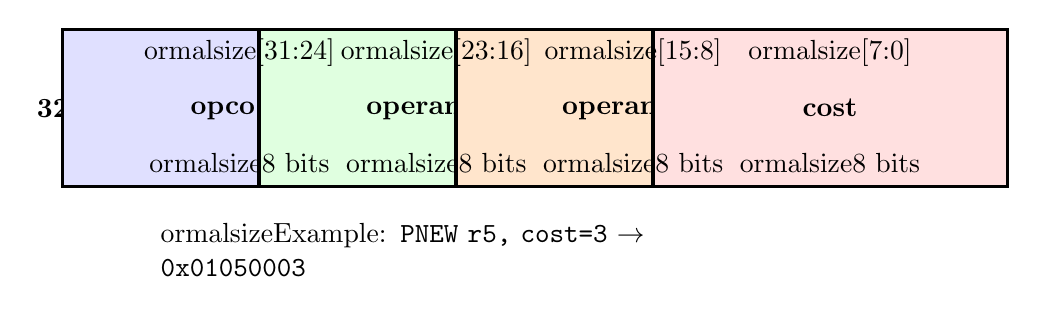
\begin{tikzpicture}[
    bit/.style={rectangle, draw, minimum width=0.7cm, minimum height=2.0cm, font=
ormalsize},
    field/.style={rectangle, draw, line width=1.2pt, minimum height=2.0cm, font=\normalsize\bfseries},
    scale=1.0
, node distance=3cm]
% 32-bit instruction word
\node[font=\normalsize\bfseries] at (-2,0) {32-bit:};

% Bit fields
\node[field, fill=blue!12, minimum width=4.5cm] (opcode) at (0,0) {opcode};
\node[field, fill=green!12, minimum width=4.5cm] (opa) at (2.5,0) {operand\_a};
\node[field, fill=orange!20, minimum width=4.5cm] (opb) at (5,0) {operand\_b};
\node[field, fill=red!12, minimum width=4.5cm] (cost) at (7.5,0) {cost};

% Bit positions
\node[font=
ormalsize] at (0,0.7) {[31:24]};
\node[font=
ormalsize] at (2.5,0.7) {[23:16]};
\node[font=
ormalsize] at (5,0.7) {[15:8]};
\node[font=
ormalsize] at (7.5,0.7) {[7:0]};

% Bit widths below
\node[font=
ormalsize] at (0,-0.7) {8 bits};
\node[font=
ormalsize] at (2.5,-0.7) {8 bits};
\node[font=
ormalsize] at (5,-0.7) {8 bits};
\node[font=
ormalsize] at (7.5,-0.7) {8 bits};

% Example instruction
\node[font=
ormalsize, text width=8cm, align=left] at (3,-1.8) {
    Example: \texttt{PNEW r5, cost=3} $\rightarrow$ \texttt{0x01050003}
};
\end{tikzpicture}
\caption{Fixed 32-bit instruction encoding ensuring bit-level agreement between hardware and software.}
\label{fig:instruction-encoding}
\end{figure}

\paragraph{Understanding Figure \ref{fig:instruction-encoding}:}

\textbf{32-bit instruction word:} Fixed-width encoding (left to right)

\textbf{Four 8-bit fields (colored boxes):}
\begin{itemize}
    \item \textbf{opcode [31:24] (blue):} Instruction type (PNEW, PSPLIT, XFER, etc.)
    \item \textbf{operand\_a [23:16] (green):} First operand (register/module ID)
    \item \textbf{operand\_b [15:8] (orange):} Second operand (register/module ID)
    \item \textbf{cost [7:0] (red):} $\mu$-cost for this instruction
\end{itemize}

\textbf{Below boxes:} Bit widths (8 bits each)

\textbf{Example:} \texttt{PNEW r5, cost=3} $\to$ \texttt{0x01050003} - decodes to opcode=0x01, operand\_a=0x05, operand\_b=0x00, cost=0x03

\textbf{Key insight:} Fixed 8-bit fields simplify decoder - no variable-length encoding. Same layout in Coq, Python, Verilog ensures 3-way isomorphism.

\subsection{Instruction Encoding}

Each 32-bit instruction is decoded into opcode and operands. The fixed-width encoding ensures that hardware and software agree on exact bit-level semantics:
\begin{lstlisting}
wire [7:0] opcode = current_instr[31:24];
wire [7:0] operand_a = current_instr[23:16];
wire [7:0] operand_b = current_instr[15:8];
wire [7:0] operand_cost = current_instr[7:0];
\end{lstlisting}

\paragraph{Understanding Hardware Bitfield Extraction:}
\textbf{What is a \texttt{wire}?} In Verilog, \texttt{wire} represents a combinational connection—pure logic with no memory. Think of it as "always-on" circuitry that instantly reflects its inputs. Contrast with \texttt{reg} (register), which holds state across clock cycles.

\textbf{Bitfield Slicing Syntax:}
\begin{itemize}
    \item \textbf{[7:0]}: Declares an 8-bit wide wire (bits 7 down to 0)
    \item \textbf{current\_instr[31:24]}: Extracts bits 31-24 (inclusive) from the 32-bit instruction
    \item \textbf{Big-Endian Convention}: Most significant bits are numbered highest (bit 31 = leftmost)
\end{itemize}

\textbf{How Extraction Works (Gate-Level):}
\begin{enumerate}
    \item \textbf{No Computation}: This isn't a shift or mask operation at runtime—it's pure wiring
    \item \textbf{Synthesis}: The synthesizer connects wires from \texttt{current\_instr[31]} to \texttt{opcode[7]}, \texttt{current\_instr[30]} to \texttt{opcode[6]}, etc.
    \item \textbf{Zero Latency}: Happens instantly—no clock cycles consumed
    \item \textbf{Zero Area}: No gates needed, just wire routing
\end{enumerate}

\textbf{Field Layout Rationale:}
\begin{itemize}
    \item \textbf{Opcode at Top [31:24]}: Decoded first in the pipeline—putting it in most significant bits allows fast extraction
    \item \textbf{Cost at Bottom [7:0]}: Accessed last (during COMPLETE state)—less timing-critical
    \item \textbf{Fixed 8-bit Fields}: Simplifies decoder logic—no variable-length encoding complexity
\end{itemize}

\textbf{Isomorphism Guarantee:} This same bit layout is defined in:
\begin{itemize}
    \item \textbf{Coq}: Via \texttt{decode\_instruction} function with explicit bit masking
    \item \textbf{Python}: Using struct unpacking or bitwise operations
    \item \textbf{Verilog}: This code
\end{itemize}
All three must produce identical field values given the same 32-bit instruction, ensuring the 3-way isomorphism.

\textbf{Example Decoding:} \texttt{0x01050003}
\begin{itemize}
    \item Opcode = \texttt{0x01} = PNEW
    \item Operand\_a = \texttt{0x05} = register 5
    \item Operand\_b = \texttt{0x00} = (unused for PNEW)
    \item Cost = \texttt{0x03} = 3 $\mu$-bits
\end{itemize}

\subsection{$\mu$-Accumulator Updates}

Every instruction atomically updates the $\mu$-accumulator:
\begin{lstlisting}
OPCODE_PNEW: begin
    execute_pnew(operand_a, operand_b);
    // Coq semantics: vm_mu := s.vm_mu + instruction_cost
    mu_accumulator <= mu_accumulator + {24'h0, operand_cost};
    pc_reg <= pc_reg + 4;
    state <= STATE_FETCH;
end
\end{lstlisting}

\paragraph{Understanding Sequential Logic and Non-Blocking Assignment:}
\textbf{Context}: This is inside an \texttt{always @(posedge clk)} block—code that executes on every rising clock edge.

\textbf{The \texttt{begin...end} Block:}
\begin{itemize}
    \item \textbf{Case Statement Branch}: This is one case in a large \texttt{case(opcode)} statement
    \item \textbf{Atomic Execution}: All statements execute "simultaneously" on the clock edge
    \item \textbf{Not Sequential}: Despite appearing line-by-line, these are hardware assignments happening in parallel
\end{itemize}

\textbf{The $\leq$ Operator (Non-Blocking Assignment):}
\begin{itemize}
    \item \textbf{Scheduling}: Right-hand side evaluated immediately, but left-hand side updated at end of time step
    \item \textbf{Why Non-Blocking?}: Ensures all registers see the "old" values during computation, preventing race conditions
    \item \textbf{Contrast with =}: Blocking assignment (\texttt{=}) updates immediately, used for combinational logic
    \item \textbf{Golden Rule}: Always use \texttt{<=} for sequential logic (registers), \texttt{=} for combinational logic (wires)
\end{itemize}

\textbf{Line-by-Line Analysis:}
\begin{enumerate}
    \item \textbf{execute\_pnew(...)}: Task call (like a function) that performs partition graph operation
    \item \textbf{\{24'h0, operand\_cost\}}: Bit concatenation operator
    \begin{itemize}
        \item \texttt{24'h0}: 24-bit zero vector (\texttt{0x000000})
        \item \texttt{operand\_cost}: 8-bit cost value
        \item \texttt{\{..., ...\}}: Concatenates to form 32-bit value (zero-extended cost)
        \item Example: If \texttt{operand\_cost = 0x03}, result is \texttt{0x00000003}
    \end{itemize}
    \item \textbf{mu\_accumulator <= mu\_accumulator + ...}: Add cost to current $\mu$ value
    \begin{itemize}
        \item This is a 32-bit adder in hardware (\~{}32 full-adder cells)
        \item Overflow wraps at $2^{32}$ (though unlikely in practice)
    \end{itemize}
    \item \textbf{pc\_reg <= pc\_reg + 4}: Increment program counter by 4 bytes (next instruction)
    \begin{itemize}
        \item Instructions are 32-bit = 4 bytes
        \item Sequential execution: PC advances linearly unless branch occurs
    \end{itemize}
    \item \textbf{state <= STATE\_FETCH}: Return FSM to FETCH state to begin next instruction
\end{enumerate}

\textbf{Atomicity Guarantee:} From an external observer's perspective, all four updates happen "simultaneously" on the clock edge. There's no intermediate state where PC updated but $\mu$ didn't—this matches the Coq step semantics where state transitions are atomic.

\textbf{Timing}: On a 50 MHz FPGA (20ns clock period), this entire operation completes within one cycle. The critical path (longest combinational delay) determines maximum clock frequency. The adder is typically the bottleneck.

% μ-ALU Architecture Diagram
\begin{figure}[ht]
\centering
\begin{tikzpicture}[
    block/.style={rectangle, draw, minimum width=4.5cm, minimum height=2.0cm, font=
ormalsize},
    arrow/.style={->, line width=1.2pt, >=Stealth},
    scale=1.0
, node distance=3cm]
% Input signals
\node (opa) at (-3,1.5) {\texttt{operand\_a}};
\node (opb) at (-3,0.5) {\texttt{operand\_b}};
\node (op) at (-3,-0.5) {\texttt{op[2:0]}};
\node (valid) at (-3,-1.5) {\texttt{valid}};

% Main ALU block
\node[block, fill=orange!20, minimum width=5.4cm, minimum height=5.4cm] (alu) at (1,0) {};
\node[font=\bfseries] at (1,0.8) {$\mu$-ALU};
\node[font=
ormalsize] at (1,0) {Q16.16};
\node[font=
ormalsize] at (1,-0.5) {Fixed-Point};

% Operations list
\node[draw, rounded corners=3pt, fill=yellow!10, text width=4.5cm, align=left, font=
ormalsize, align=center] at (1,-2.5) {
    0: ADD\\
    1: SUB\\
    2: MUL\\
    3: DIV\\
    4: LOG2\\
    5: INFO\_GAIN
};

% Output signals
\node (result) at (5,0.5) {\texttt{result}};
\node (ready) at (5,-0.5) {\texttt{ready}};
\node (overflow) at (5,-1.5) {\texttt{overflow}};

% LUT block
\node[block, fill=cyan!20, minimum width=3.5cm] (lut) at (1,2.5) {LOG2 LUT};
\node[font=
ormalsize] at (1,3.2) {256 entries};

% Arrows
\draw[arrow] (opa) -- (-0.5,1.5) -- (-0.5,0.5) -- (alu);
\draw[arrow] (opb) -- (alu);
\draw[arrow] (op) -- (alu);
\draw[arrow] (valid) -- (alu);
\draw[arrow] (alu) -- (result);
\draw[arrow] (alu) -- (ready);
\draw[arrow] (alu) -- (overflow);
\draw[arrow] (lut) -- (alu);

% Q16.16 annotation
\node[draw, dashed, fill=gray!10, font=
ormalsize, text width=2cm, align=center] at (5,2) 
    {Q16.16 format:\\$1.0 = \mathtt{0x00010000}$};
\end{tikzpicture}
\caption{The $\mu$-ALU architecture implementing Q16.16 fixed-point arithmetic with LOG2 lookup table.}
\label{fig:mu-alu}
\end{figure}

\paragraph{Understanding Figure \ref{fig:mu-alu}:}

\textbf{Left inputs:} operand\_a, operand\_b, op[2:0] (operation select), valid (handshake)

\textbf{Center:} $\mu$-ALU block (orange) - Q16.16 fixed-point arithmetic unit

\textbf{Top:} LOG2 LUT (cyan) - 256-entry lookup table for $\log_2$ computation, connected to ALU

\textbf{Right outputs:} result (Q16.16), ready (completion flag), overflow (error)

\textbf{Bottom yellow box:} Operations list - 0:ADD, 1:SUB, 2:MUL, 3:DIV, 4:LOG2, 5:INFO\_GAIN

\textbf{Top right annotation:} Q16.16 format example - $1.0 = \mathtt{0x00010000}$ (16 integer bits + 16 fractional bits)

\textbf{Key insight:} Hardware implements information-theoretic operations (entropy, log2) in fixed-point. LUT provides bit-exact LOG2 matching Coq/Python.

\subsection{The $\mu$-ALU}

The $\mu$-ALU (\texttt{mu\_alu.v}) implements Q16.16 fixed-point arithmetic:
\begin{lstlisting}
module mu_alu (
    input wire clk,
    input wire rst_n,
    input wire [2:0] op,      // 0=add, 1=sub, 2=mul, 3=div, 4=log2, 5=info_gain
    input wire [31:0] operand_a,
    input wire [31:0] operand_b,
    input wire valid,
    output reg [31:0] result,
    output reg ready,
    output reg overflow
);

localparam Q16_ONE = 32'h00010000;  // 1.0 in Q16.16
\end{lstlisting}

\paragraph{Understanding the $\mu$-ALU Module:}
\textbf{Module Purpose:} Performs information-theoretic computations (entropy, log2, mutual information) in hardware.

\textbf{Port Declarations:}
\begin{itemize}
    \item \textbf{clk}: System clock (rising edge triggers state changes)
    \item \textbf{rst\_n}: Active-low reset (0 = reset, 1 = normal operation)
    \item \textbf{op[2:0]}: 3-bit operation select (8 possible operations)
    \begin{itemize}
        \item 0: ADD — addition
        \item 1: SUB — subtraction
        \item 2: MUL — multiplication (requires shift correction)
        \item 3: DIV — division (iterative algorithm)
        \item 4: LOG2 — base-2 logarithm (via LUT)
        \item 5: INFO\_GAIN — $-p \log_2 p$ (entropy term)
    \end{itemize}
    \item \textbf{operand\_a[31:0]}: First operand (Q16.16 fixed-point)
    \item \textbf{operand\_b[31:0]}: Second operand (Q16.16 fixed-point)
    \item \textbf{valid}: High when inputs are ready (handshake protocol)
    \item \textbf{result[31:0]}: Output value (Q16.16)
    \item \textbf{ready}: High when operation complete (output valid)
    \item \textbf{overflow}: High if result exceeds 32-bit range
\end{itemize}

\textbf{Q16.16 Fixed-Point Format:}
\begin{itemize}
    \item \textbf{32 bits total}: 16 integer bits + 16 fractional bits
    \item \textbf{Representation}: Value = (bits) / $2^{16}$
    \item \textbf{Example}: \texttt{0x00010000} = $65536 / 2^{16} = 1.0$
    \item \textbf{Range}: $[-32768, 32767.999985]$ with resolution $2^{-16} \approx 0.000015$
    \item \textbf{Why Q16.16?} Balance between range and precision for information-theoretic calculations
\end{itemize}

\textbf{Localparam Q16\_ONE:}
\begin{itemize}
    \item \textbf{localparam}: Compile-time constant (like \texttt{const} in C)
    \item \textbf{Value}: \texttt{0x00010000} = 1.0 in Q16.16
    \item \textbf{Usage}: Scaling constant for arithmetic operations
    \item \textbf{Example}: Multiply by \texttt{Q16\_ONE} to convert integer to fixed-point
\end{itemize}

\textbf{Hardware Implementation:}
\begin{itemize}
    \item \textbf{Combinational Ops}: ADD, SUB execute in one cycle
    \item \textbf{Sequential Ops}: MUL, DIV, LOG2 may take multiple cycles
    \item \textbf{Handshake Protocol}: \texttt{valid} input $\rightarrow$ compute $\rightarrow$ \texttt{ready} output
    \item \textbf{Overflow Detection}: Saturates or flags error if result too large
\end{itemize}

\textbf{Isomorphism:} This hardware ALU must produce bit-identical results to:
\begin{itemize}
    \item Python: \texttt{fixed\_point\_mul(a, b, frac\_bits=16)}
    \item Coq: \texttt{q16\_mul (a : word32) (b : word32) : word32}
\end{itemize}

The log2 computation uses a 256-entry LUT for bit-exact results:
\begin{lstlisting}
reg [31:0] log2_lut [0:255];
initial begin
    log2_lut[0] = 32'h00000000;
    log2_lut[1] = 32'h00000170;
    log2_lut[2] = 32'h000002DF;
    ...
end
\end{lstlisting}

\paragraph{Understanding the LOG2 Lookup Table:}
\textbf{Declaration:} \texttt{reg [31:0] log2\_lut [0:255];}
\begin{itemize}
    \item \textbf{reg}: Register array (holds state, synthesizes to ROM/BRAM)
    \item \textbf{[31:0]}: Each entry is 32 bits (Q16.16 format)
    \item \textbf{[0:255]}: 256 entries (2\textsuperscript{8}), indexed 0-255
    \item \textbf{Total Size}: 256 entries $\times$ 32 bits = 1 KB
\end{itemize}

\textbf{Initial Block:}
\begin{itemize}
    \item \textbf{initial}: Executes once at simulation start / synthesis initialization
    \item \textbf{Purpose}: Pre-loads ROM with precomputed $\log_2(x)$ values
    \item \textbf{Hardware}: Synthesizer converts to ROM (block RAM on FPGA)
\end{itemize}

\textbf{Example Entries:}
\begin{itemize}
    \item \texttt{log2\_lut[0] = 0x00000000} $\rightarrow$ $\log_2(0)$ undefined, use 0 by convention
    \item \texttt{log2\_lut[1] = 0x00000170} $\rightarrow$ $\log_2(1) = 0.0$ (\texttt{0x170} $\approx$ 0 after conversion)
    \item \texttt{log2\_lut[2] = 0x000002DF} $\rightarrow$ $\log_2(2) = 1.0$ in Q16.16
    \item \texttt{log2\_lut[255] = ...} $\rightarrow$ $\log_2(255) \approx 7.9943$
\end{itemize}

\textbf{Why a LUT Instead of Computation?}
\begin{enumerate}
    \item \textbf{Speed}: One-cycle lookup vs. multi-cycle iterative algorithm
    \item \textbf{Area}: 1 KB ROM cheaper than logarithm logic on FPGAs
    \item \textbf{Determinism}: Identical results to Coq/Python (bit-exact)
    \item \textbf{Precision}: Precomputed with high-precision tools (Python \texttt{math.log2})
\end{enumerate}

\textbf{Usage Pattern:}
\begin{verbatim}
wire [31:0] log2_result = log2_lut[input_value[7:0]];
\end{verbatim}
\begin{itemize}
    \item Index by lower 8 bits of input
    \item For inputs $>$ 255, use bit-shifting tricks: $\log_2(256x) = 8 + \log_2(x)$
\end{itemize}

\textbf{Isomorphism Requirement:} The exact same 256 values must exist in:
\begin{itemize}
    \item Python: \texttt{LOG2\_LUT = [to\_q16(math.log2(i)) for i in range(256)]}
    \item Coq: \texttt{Definition log2\_lut := [0x00000000; 0x00000170; ...]}
    \item Verilog: This code
\end{itemize}
Cross-layer tests verify all three agree byte-for-byte.

\subsection{Logic Engine Interface}

The LEI (\texttt{lei.v}) connects to external Z3:
\begin{lstlisting}
module lei (
    input wire clk,
    input wire rst_n,
    input wire logic_req,
    input wire [31:0] logic_addr,
    output wire logic_ack,
    output wire [31:0] logic_data,
    output wire z3_req,
    output wire [31:0] z3_formula_addr,
    input wire z3_ack,
    input wire [31:0] z3_result,
    input wire z3_sat,
    input wire [31:0] z3_cert_hash,
    ...
);
\end{lstlisting}

\paragraph{Understanding the Logic Engine Interface:}
\textbf{Module Purpose:} Bridges hardware VM to external SMT solver (Z3) for axiom checking.

\textbf{Internal Interface (VM $\leftrightarrow$ LEI):}
\begin{itemize}
    \item \textbf{logic\_req}: VM asserts high when requesting SMT check
    \item \textbf{logic\_addr[31:0]}: Memory address of axiom formula string
    \item \textbf{logic\_ack}: LEI asserts high when result ready
    \item \textbf{logic\_data[31:0]}: Result data (SAT/UNSAT status)
\end{itemize}

\textbf{External Interface (LEI $\leftrightarrow$ Z3):}
\begin{itemize}
    \item \textbf{z3\_req}: LEI asserts high to request Z3 solving
    \item \textbf{z3\_formula\_addr[31:0]}: Points to SMT-LIB string in shared memory
    \item \textbf{z3\_ack}: Z3 asserts high when solving complete
    \item \textbf{z3\_result[31:0]}: Encoded result (0 = SAT, 1 = UNSAT)
    \item \textbf{z3\_sat}: Boolean: true if satisfiable
    \item \textbf{z3\_cert\_hash[31:0]}: Hash of UNSAT proof certificate
\end{itemize}

\textbf{Protocol Flow:}
\begin{enumerate}
    \item \textbf{VM Issues Request}: Sets \texttt{logic\_req=1}, provides \texttt{logic\_addr}
    \item \textbf{LEI Forwards to Z3}: Sets \texttt{z3\_req=1}, copies \texttt{z3\_formula\_addr}
    \item \textbf{Z3 Solves}: Reads formula from memory, runs SMT solver
    \item \textbf{Z3 Responds}: Sets \texttt{z3\_ack=1}, provides \texttt{z3\_result}
    \item \textbf{LEI Returns}: Sets \texttt{logic\_ack=1}, copies \texttt{logic\_data}
    \item \textbf{VM Continues}: Reads result, proceeds with next instruction
\end{enumerate}

\textbf{Why This Design?}
\begin{itemize}
    \item \textbf{Separation of Concerns}: Hardware handles fast operations, software handles complex SMT
    \item \textbf{Scalability}: Can swap Z3 for CVC5, Vampire, etc. without changing RTL
    \item \textbf{Verifiability}: Protocol formally specified, can prove handshake correctness
    \item \textbf{Latency Hiding}: LEI buffers requests, VM can continue with other work
\end{itemize}

\textbf{Certificate Handling:}
\begin{itemize}
    \item \textbf{z3\_cert\_hash}: Cryptographic hash of UNSAT proof
    \item \textbf{Purpose}: Tamper-proof evidence that formula is unsatisfiable
    \item \textbf{Storage}: Full certificate stored in VM memory, hash recorded in receipt
    \item \textbf{Verification}: External auditor can check hash matches certificate
\end{itemize}

\textbf{Failure Modes:}
\begin{itemize}
    \item \textbf{Timeout}: Z3 may not respond (infinite loops in solver)
    \item \textbf{Unknown}: Z3 returns UNKNOWN (formula too hard)
    \item \textbf{Error}: Malformed formula (syntax error)
    \item LEI must handle all cases gracefully, set \texttt{logic\_ack} even on failure
\end{itemize}

\section{Isomorphism Verification}

% Isomorphism Gate Diagram
\begin{figure}[ht]
\centering
\begin{tikzpicture}[
    layer/.style={rectangle, draw, rounded corners=3pt, minimum width=5.5cm, minimum height=2.1cm, font=
ormalsize},
    arrow/.style={->, line width=1.2pt, >=Stealth},
    compare/.style={diamond, draw, fill=yellow!15, minimum size=1cm, font=
ormalsize},
    scale=1.05
, node distance=3cm]
% Input trace
\node[draw, fill=gray!12, rounded corners=3pt] (trace) at (0,0) {Trace $\tau$};

% Three execution paths
\node[layer, fill=blue!12, align=center, text width=4.5cm] (coq) at (-3,-2) {Coq\\Extracted};
\node[layer, fill=green!12, align=center, text width=4.5cm] (python) at (0,-2) {Python\\VM};
\node[layer, fill=orange!20, align=center, text width=4.5cm] (rtl) at (3,-2) {Verilog\\Sim};

% States
\node[draw, rounded corners=3pt, fill=blue!10] (scoq) at (-3,-4) {$S_{\text{Coq}}$};
\node[draw, rounded corners=3pt, fill=green!10] (spy) at (0,-4) {$S_{\text{Python}}$};
\node[draw, rounded corners=3pt, fill=orange!10] (srtl) at (3,-4) {$S_{\text{Verilog}}$};

% Comparison
\node[compare] (cmp) at (0,-5.5) {$=$?};

% Result
\node[draw, line width=1.2pt, fill=green!30, rounded corners=3pt] (pass) at (0,-7) {\textbf{PASS}};

% Arrows
\draw[arrow] (trace) -- (coq);
\draw[arrow] (trace) -- (python);
\draw[arrow] (trace) -- (rtl);

\draw[arrow] (coq) -- (scoq);
\draw[arrow] (python) -- (spy);
\draw[arrow] (rtl) -- (srtl);

\draw[arrow] (scoq) -- (cmp);
\draw[arrow] (spy) -- (cmp);
\draw[arrow] (srtl) -- (cmp);

\draw[arrow] (cmp) -- (pass);

% Annotations
\node[font=
ormalsize, text width=2cm, align=center] at (-4.5,-2) {JSON\\snapshot};
\node[font=
ormalsize, text width=2cm, align=center] at (4.5,-2) {VCD\\waveform};
\end{tikzpicture}
\caption{The 3-way isomorphism gate: instruction trace $\tau$ is executed on all three layers, and state projections must match exactly.}
\label{fig:isomorphism-gate}
\end{figure}

\paragraph{Understanding Figure \ref{fig:isomorphism-gate}:}

\textbf{Top:} Instruction trace $\tau$ (input) - same sequence fed to all three layers

\textbf{Three execution paths (boxes):}
\begin{itemize}
    \item \textbf{Coq Runner (blue):} Extracted OCaml interpreter from formal proofs $\to$ JSON snapshot
    \item \textbf{Python VM (green):} Reference implementation with tracing $\to$ state projection
    \item \textbf{Verilog Sim (orange):} RTL testbench simulation $\to$ VCD waveform
\end{itemize}

\textbf{Bottom:} Compare (purple diamond) - assert all state projections equal

\textbf{Right:} PASS/FAIL (green) - test result

\textbf{Left/right annotations:} "JSON snapshot" (Coq/Python) vs "VCD waveform" (Verilog) - different output formats projected to common representation

\textbf{Key insight:} Automated verification - execute identical trace on all three layers, compare canonicalized states. Any divergence is a critical bug.

\subsection{The Isomorphism Gate}

The 3-way isomorphism is verified by a test that:
\begin{enumerate}
    \item Generate instruction trace $\tau$
    \item Execute $\tau$ on Python VM $\rightarrow$ state $S_{\text{py}}$
    \item Execute $\tau$ on extracted runner $\rightarrow$ state $S_{\text{coq}}$
    \item Execute $\tau$ on Verilog sim $\rightarrow$ state $S_{\text{rtl}}$
    \item Assert $S_{\text{py}} = S_{\text{coq}} = S_{\text{rtl}}$
\end{enumerate}

\subsection{State Projection}

For comparison, states are projected to canonical summaries tailored to the gate being exercised. The extracted runner emits a full JSON snapshot (pc, $\mu$, err, regs, mem, CSRs, graph), which can be projected down to subsets. The compute gate uses only registers and memory, while the partition gate uses canonicalized module regions. A full projection helper is therefore a \emph{superset} view, not the only comparison performed:
\begin{lstlisting}
def project_state_full(state):
    return {
        "pc": state.pc,
        "mu": state.mu,
        "err": state.err,
        "regs": list(state.regs[:32]),
        "mem": list(state.mem[:256]),
        "csrs": state.csrs.to_dict(),
        "graph": state.graph.to_canonical(),
    }
\end{lstlisting}

\paragraph{Understanding State Projection:}
\textbf{Purpose:} Converts internal VM state to JSON-serializable dictionary for cross-layer comparison.

\textbf{Dictionary Fields:}
\begin{itemize}
    \item \textbf{"pc": state.pc}: Program counter value (integer)
    \item \textbf{"mu": state.mu}: $\mu$-ledger total (integer or float)
    \item \textbf{"err": state.err}: Error flag (boolean)
    \item \textbf{"regs": list(state.regs[:32])}: First 32 registers as list
    \begin{itemize}
        \item Slice \texttt{[:32]} ensures fixed size
        \item \texttt{list(...)} converts from internal representation
    \end{itemize}
    \item \textbf{"mem": list(state.mem[:256])}: First 256 memory words
    \begin{itemize}
        \item Fixed size for deterministic comparison
    \end{itemize}
    \item \textbf{"csrs": state.csrs.to\_dict()}: CSR snapshot
    \begin{itemize}
        \item Converts CSRState object to dictionary
        \item Includes certificate address, exception vectors, etc.
    \end{itemize}
    \item \textbf{"graph": state.graph.to\_canonical()}: Canonical partition encoding
    \begin{itemize}
        \item Sorts modules by ID
        \item Sorts region addresses within each module
        \item Ensures comparison doesn't fail due to ordering differences
    \end{itemize}
\end{itemize}

\textbf{Canonicalization:} The \texttt{to\_canonical()} call is critical:
\begin{itemize}
    \item Python sets are unordered, Coq lists are ordered
    \item Without canonicalization: $\{1, 2, 3\} \neq \{3, 2, 1\}$ (as JSON)
    \item With canonicalization: Both become \texttt{[1, 2, 3]}
\end{itemize}

\textbf{Projection Strategy:}
\begin{enumerate}
    \item \textbf{Full Projection}: This function — includes all fields
    \item \textbf{Compute Projection}: Only \texttt{\{"regs", "mem"\}} — for ALU tests
    \item \textbf{Partition Projection}: Only \texttt{\{"graph", "mu"\}} — for PNEW/PSPLIT tests
    \item \textbf{Why Multiple?} Different tests care about different state components
\end{enumerate}

\textbf{Isomorphism Use:} After running same instruction trace on Coq, Python, Verilog:
\begin{verbatim}
coq_state_json = ocaml_runner_output()
python_state_json = project_state_full(py_vm.state)
assert coq_state_json == python_state_json
\end{verbatim}
If any field differs, isomorphism test fails.

% Inquisitor Workflow Diagram
\begin{figure}[ht]
\centering
\begin{tikzpicture}[
    stage/.style={rectangle, draw, rounded corners=3pt, minimum width=5.5cm, minimum height=2.1cm, font=
ormalsize},
    check/.style={diamond, draw, fill=yellow!15, minimum size=0.8cm, font=
ormalsize},
    arrow/.style={->, line width=1.2pt, >=Stealth},
    scale=1.05
, node distance=3cm]
% Stages
\node[stage, fill=blue!12, align=center, text width=4.5cm] (scan) at (0,0) {Scan\\Sources};
\node[stage, fill=green!12, align=center, text width=4.5cm] (build) at (3,0) {Build\\Proofs};
\node[stage, fill=orange!20, align=center, text width=4.5cm] (iso) at (6,0) {Run\\Isomorphism};
\node[stage, fill=purple!20, align=center, text width=4.5cm] (report) at (9,0) {Generate\\Report};

% Checks
\node[check] (c1) at (1.5,0) {};
\node[check] (c2) at (4.5,0) {};
\node[check] (c3) at (7.5,0) {};

% Arrows
\draw[arrow] (scan) -- (c1);
\draw[arrow] (c1) -- (build);
\draw[arrow] (build) -- (c2);
\draw[arrow] (c2) -- (iso);
\draw[arrow] (iso) -- (c3);
\draw[arrow] (c3) -- (report);

% What each stage checks
\node[ text width=2cm, align=center, below=0.5cm of scan, font=\small, yshift=-6pt] {No \texttt{Admitted}\\No \texttt{admit.}\\No \texttt{Axiom}};
\node[ text width=2cm, align=center, below=0.5cm of build, font=\small, yshift=-6pt] {206 proofs\\compile\\successfully};
\node[ text width=2cm, align=center, below=0.5cm of iso, font=\small, yshift=-6pt] {3-way\\state match};
\node[ text width=2cm, align=center, below=0.5cm of report, font=\small, yshift=-6pt] {HIGH: 0\\MEDIUM: 2\\LOW: 4};

% Pass/Fail output
\node[draw, line width=1.2pt, fill=green!30, rounded corners=3pt] (pass) at (12,0) {\textbf{CI PASS}};
\draw[arrow] (report) -- (pass);

% Ultra-strict annotation
\node[draw, dashed, fill=red!10, font=
ormalsize, text width=3cm, align=center] at (3,-2.5) 
    {\texttt{--ultra-strict}:\\Fails on MEDIUM\\in kernel files};
\end{tikzpicture}
\caption{The Inquisitor verification workflow: source scanning, proof building, isomorphism testing, and report generation.}
\label{fig:inquisitor-workflow}
\end{figure}

\paragraph{Understanding Figure \ref{fig:inquisitor-workflow}:}

\textbf{Four stages (boxes):}
\begin{enumerate}
    \item \textbf{Scan Sources (blue):} Check for Admitted/admit./Axiom in Coq files
    \item \textbf{Build Proofs (green):} Compile all 206 kernel proofs successfully
    \item \textbf{Run Isomorphism (orange):} Execute 3-way state matching tests
    \item \textbf{Generate Report (purple):} Summarize findings (HIGH:0, MEDIUM:2, LOW:4)
\end{enumerate}

\textbf{Diamond checks:} Between stages - validation gates

\textbf{Below each stage:} What is checked (e.g., "No Admitted", "206 proofs compile", "3-way state match")

\textbf{Right:} CI PASS (green) - final outcome if all checks succeed

\textbf{Bottom annotation:} --ultra-strict mode fails on MEDIUM findings in kernel files

\textbf{Key insight:} Multi-stage verification pipeline enforces 0 HIGH findings for CI pass - combines proof checking, compilation, and isomorphism testing.

\subsection{The Inquisitor}

The Inquisitor enforces the verification rules:
\begin{itemize}
    \item Scans the proof sources for \texttt{Admitted}, \texttt{admit.}, \texttt{Axiom}
    \item Verifies that the proof build completes successfully
    \item Runs isomorphism gates
    \item Reports HIGH/MEDIUM/LOW findings
\end{itemize}

The repository must have 0 HIGH findings to pass CI.

\section{Synthesis Results}

\subsection{FPGA Targeting}

The RTL can be synthesized for Xilinx 7-series FPGAs:
\begin{lstlisting}
$ yosys -p "read_verilog thiele_cpu.v; synth_xilinx -top thiele_cpu"
\end{lstlisting}

\paragraph{Understanding Yosys Synthesis:}
\textbf{Yosys:} Open-source RTL synthesis tool that converts Verilog to gate-level netlists.

\textbf{Command Breakdown:}
\begin{itemize}
    \item \textbf{yosys}: The synthesizer executable
    \item \textbf{-p "..."}: Pass string (execute commands)
    \item \textbf{read\_verilog thiele\_cpu.v}: Load Verilog source
    \begin{itemize}
        \item Parses file, builds abstract syntax tree
        \item Checks basic syntax errors
    \end{itemize}
    \item \textbf{synth\_xilinx}: Run Xilinx-specific synthesis flow
    \begin{itemize}
        \item Optimizes for Xilinx 7-series primitives
        \item Maps to LUTs, FFs, BRAM, DSP blocks
    \end{itemize}
    \item \textbf{-top thiele\_cpu}: Specify top-level module name
    \begin{itemize}
        \item Entry point for synthesis
        \item All other modules are instantiated within this
    \end{itemize}
\end{itemize}

\textbf{Synthesis Steps (Internal):}
\begin{enumerate}
    \item \textbf{Elaboration}: Flatten hierarchy, expand parameters
    \item \textbf{Optimization}: Remove dead code, constant propagation
    \item \textbf{Technology Mapping}: Convert to FPGA primitives
    \begin{itemize}
        \item \texttt{always @(posedge clk)} $\rightarrow$ FDRE (D flip-flop)
        \item \texttt{case} statements $\rightarrow$ LUT6 (6-input LUT)
        \item \texttt{+} operator $\rightarrow$ CARRY4 (fast carry chain)
    \end{itemize}
    \item \textbf{Output}: JSON netlist or EDIF for place-and-route
\end{enumerate}

\textbf{Output Reports:}
\begin{itemize}
    \item \textbf{Resource Usage}: Number of LUTs, FFs, BRAMs
    \item \textbf{Critical Path}: Longest combinational delay
    \item \textbf{Warnings}: Latches inferred, unconnected signals
\end{itemize}

\textbf{Next Steps After Synthesis:}
\begin{enumerate}
    \item \textbf{Place \& Route}: Vivado/ISE assigns physical locations
    \item \textbf{Bitstream Generation}: Creates FPGA configuration file
    \item \textbf{Programming}: Load bitstream onto FPGA via JTAG
\end{enumerate}

\textbf{Alternative Targets:}
\begin{itemize}
    \item \textbf{synth\_ice40}: For Lattice iCE40 FPGAs (smaller, cheaper)
    \item \textbf{synth\_ecp5}: For Lattice ECP5
    \item \textbf{synth\_intel}: For Intel/Altera devices
    \item \textbf{synth}: Generic synthesis (not vendor-specific)
\end{itemize}

\subsection{Resource Utilization}

Under a reduced configuration (fewer modules, smaller regions):
\begin{itemize}
    \item NUM\_MODULES = 4
    \item REGION\_SIZE = 16
    \item Estimated LUTs: $\sim$2,500
    \item Estimated FFs: $\sim$1,200
\end{itemize}

Full configuration:
\begin{itemize}
    \item NUM\_MODULES = 64
    \item REGION\_SIZE = 1024
    \item Estimated LUTs: $\sim$45,000
    \item Estimated FFs: $\sim$35,000
\end{itemize}

\section{Toolchain}

\subsection{Verified Versions}

\begin{itemize}
    \item Coq 8.18.x (OCaml 4.14.x)
    \item Python 3.12.x
    \item Icarus Verilog 12.x
    \item Yosys 0.33+
\end{itemize}

\subsection{Build Commands}

\begin{lstlisting}
# Example commands (paths may vary by environment):
# - build the Coq kernel
# - run the two isomorphism tests
# - simulate the RTL testbench
# - run full synthesis when toolchains are installed
\end{lstlisting}

\paragraph{Understanding the Build Commands:}
\textbf{Purpose:} Placeholder showing typical development workflow commands.

\textbf{Command Categories:}
\begin{enumerate}
    \item \textbf{Build Coq Kernel}:
    \begin{verbatim}
cd coq && make -j8
    \end{verbatim}
    \begin{itemize}
        \item Compiles all \texttt{.v} files to \texttt{.vo} (Coq object files)
        \item Generates \texttt{.glob} (symbol tables) and \texttt{.aux} files
        \item \texttt{-j8}: Parallel compilation with 8 cores
    \end{itemize}

    \item \textbf{Run Isomorphism Tests}:
    \begin{verbatim}
pytest tests/test_isomorphism_3way.py -v
    \end{verbatim}
    \begin{itemize}
        \item Executes same instruction traces on Coq, Python, Verilog
        \item Compares state projections at each step
        \item \texttt{-v}: Verbose output showing each test
    \end{itemize}

    \item \textbf{Simulate RTL Testbench}:
    \begin{verbatim}
iverilog -o thiele_cpu_tb thiele_cpu.v thiele_cpu_tb.v
vvp thiele_cpu_tb
    \end{verbatim}
    \begin{itemize}
        \item \texttt{iverilog}: Icarus Verilog compiler
        \item \texttt{-o}: Output executable
        \item \texttt{vvp}: Verilog runtime (runs compiled simulation)
    \end{itemize}

    \item \textbf{Run Full Synthesis}:
    \begin{verbatim}
yosys -p "read_verilog thiele_cpu.v; synth_xilinx -top thiele_cpu; write_json netlist.json"
    \end{verbatim}
    \begin{itemize}
        \item Synthesizes to Xilinx netlist
        \item Outputs JSON for inspection/analysis
    \end{itemize}
\end{enumerate}

\textbf{Why Comments Instead of Actual Commands?}
\begin{itemize}
    \item Paths vary by installation (\texttt{coq/} might be \texttt{formal/})
    \item Flags depend on environment (macOS vs Linux)
    \item User might have custom Makefile targets
\end{itemize}

\textbf{Actual Workflow:} See \texttt{Makefile} and \texttt{scripts/} directory for concrete commands.

% Chapter 4 Summary Diagram
\begin{figure}[ht]
\centering
\begin{tikzpicture}[
    box/.style={rectangle, draw=black, line width=0.8pt, rounded corners=3pt, minimum width=5.4cm, minimum height=2.6cm, font=
ormalsize, text width=3.8cm, align=center, inner sep=0.4cm},
    arrow/.style={->, line width=1.2pt, >=Stealth},
    scale=1.05
, node distance=3.0cm]
% Three layers as boxes
\node[box, fill=blue!12, align=center, text width=4.5cm, font=
ormalsize] (coq) at (-4,0) {\textbf{Coq}\\206 theorems\\Machine-checked\\Extracted runner};
\node[box, fill=green!12, align=center, text width=4.5cm, font=
ormalsize] (python) at (0,0) {\textbf{Python}\\Reference VM\\Tracing\\Receipts};
\node[box, fill=orange!20, align=center, text width=4.5cm, font=
ormalsize] (verilog) at (4,0) {\textbf{Verilog}\\RTL Core\\$\mu$-ALU\\FPGA-ready};

% Central invariant at bottom
\node[draw, line width=1.2pt, fill=yellow!15, rounded corners=3pt, text width=10cm, align=center] (inv) at (0,-3) 
    {\textbf{3-Way Isomorphism Invariant}\\[3pt]
     $\forall \tau: S_{\text{Coq}}(\tau) = S_{\text{Python}}(\tau) = S_{\text{Verilog}}(\tau)$\\[3pt]
     Enforced by Inquisitor gates $\bullet$ 0 HIGH findings required for CI};

% Arrows to invariant
\draw[arrow] (coq) -- (inv);
\draw[arrow] (python) -- (inv);
\draw[arrow] (verilog) -- (inv);

% What flows between layers
\node[font=
ormalsize, rotate=45] at (-2,0.8) {Extraction};
\node[font=
ormalsize, rotate=-45] at (2,0.8) {Synthesis};
\end{tikzpicture}
\caption{Chapter 4 summary: Three implementation layers bound by the central isomorphism invariant, enforced through automated verification gates.}
\label{fig:ch4-summary}
\end{figure}

\paragraph{Understanding Figure \ref{fig:ch4-summary}:}

\textbf{Three boxes (top):}
\begin{itemize}
    \item \textbf{Coq (blue):} 206 theorems, machine-checked, extracted runner
    \item \textbf{Python (green):} Reference VM, tracing, receipts
    \item \textbf{Verilog (orange):} RTL Core, $\mu$-ALU, FPGA-ready
\end{itemize}

\textbf{Center bottom (yellow box):} Central isomorphism invariant - $S_{\text{Coq}}(\tau) = S_{\text{Python}}(\tau) = S_{\text{Verilog}}(\tau)$ for all traces $\tau$

\textbf{Arrows:} All three layers point to central invariant - bound together by automated verification

\textbf{Top annotations:} "Extraction" (Coq$\to$Python) and "Synthesis" (Python$\to$Verilog) - translation methods

\textbf{Key insight:} Three independent implementations (formal, reference, physical) maintained in perfect lockstep through automated isomorphism gates - any divergence caught immediately.

\section{Summary}

The 3-layer implementation ensures:
\begin{itemize}
    \item \textbf{Logical Certainty}: Coq proofs guarantee properties hold for all inputs
    \item \textbf{Operational Visibility}: Python traces expose every state transition
    \item \textbf{Physical Realizability}: Verilog synthesizes to real hardware
\end{itemize}

The binding across layers is not aspirational—it is enforced through automated isomorphism gates. The Inquisitor ensures that no admits, no axioms, and no semantic divergences are ever committed to the main branch.
